%========================%
%    Initial Settings    %
%========================%
%  ignore all lines up   %
%       to line 78       %
%========================%

\documentclass{article}
\usepackage[utf8]{inputenc}
\usepackage[american]{babel}
\usepackage{listings}
\usepackage{titlesec}
\usepackage{hanging}
\usepackage{indentfirst}
\usepackage{setspace}
\usepackage{float}
\usepackage{multirow}
\usepackage{mathrsfs}
\usepackage{caption}
\usepackage{tocbasic}
\usepackage[toc,page]{appendix}
\DeclareTOCStyleEntry[beforeskip=.1em plus 1pt, pagenumberformat=\textbf]{tocline}{section}
\usepackage{adjustbox}
\usepackage[american]{babel}
\usepackage[style=apa]{biblatex}
\addbibresource{citations.bib}
\usepackage{csquotes}
\setlength{\parindent}{4em}
\setlength{\parskip}{0.5em}
\usepackage{array}
\usepackage{hyperref}
\onehalfspacing
\hypersetup{
    colorlinks=false,
    linkcolor=black,
    filecolor=black,
    urlcolor=black,
}
\newcommand{\MYhref}[3][blue]{\href{#2}{\color{#1}{#3}}}%
\urlstyle{same}
\usepackage[letterpaper, portrait, margin=1in]{geometry}
\usepackage{graphicx}
\graphicspath{ {images/} }
\usepackage{array}
\newcolumntype{L}[1]{>{\raggedright\let\newline\\\arraybackslash\hspace{0pt}}m{#1}}
\newcolumntype{C}[1]{>{\centering\let\newline\\\arraybackslash\hspace{0pt}}m{#1}}
\newcolumntype{R}[1]{>{\raggedleft\let\newline\\\arraybackslash\hspace{0pt}}m{#1}}
\titleclass{\subsubsubsection}{straight}[\subsection]

\newcounter{subsubsubsection}[subsubsection]
\renewcommand\thesubsubsubsection{\thesubsubsection.\arabic{subsubsubsection}}

\titleformat{\subsubsubsection}
  {\normalfont\normalsize\bfseries}{\thesubsubsubsection}{1em}{}
\titlespacing*{\subsubsubsection}
{0pt}{3.25ex plus 1ex minus .2ex}{1.5ex plus .2ex}

\makeatletter
\renewcommand\paragraph{\@startsection{paragraph}{5}{\z@}%
  {3.25ex \@plus1ex \@minus.2ex}%
  {-1em}%
  {\normalfont\normalsize\bfseries}}
\renewcommand\subparagraph{\@startsection{subparagraph}{6}{\parindent}%
  {3.25ex \@plus1ex \@minus .2ex}%
  {-1em}%
  {\normalfont\normalsize\bfseries}}
\def\toclevel@subsubsubsection{4}
\def\toclevel@paragraph{5}
\def\toclevel@paragraph{6}
\def\l@subsubsubsection{\@dottedtocline{4}{7em}{4em}}
\def\l@paragraph{\@dottedtocline{5}{10em}{5em}}
\def\l@subparagraph{\@dottedtocline{6}{14em}{6em}}
\def\code#1{\texttt{#1}}
\makeatother

\setcounter{secnumdepth}{4}
\setcounter{tocdepth}{4}

\renewcommand{\contentsname}{Table of Contents}
\renewcommand{\listtablename}{Tables}
\renewcommand{\listfigurename}{Figures}

%========================%
% Beginning of Document  %
%========================%

\begin{document} 

%========================%
%     General Note       %
%========================%
%  Start new line: '\\'  %
%  Start new paragraph:  %
%         '\par'         %
%========================%

%========================%
%       Title Page       %
%========================%

\pagenumbering{gobble} % Disable page number on title page
\begin{center}
    \Huge{\textbf{Creating an End-to-end Testing Framework for an Open Source Minecraft Server}} \\ % Input title of MQP
    \vspace{10mm} % Add vertical space between sections
    \large{
    A Major Qualifying Project (MQP) Report \\
    Submitted to the Faculty of \\
    WORCESTER POLYTECHNIC INSTITUTE \\
    in partial fulfillment of the requirements \\
    for the Degree of Bachelor of Science in \\
    } % Do not edit this portion
    \Large{
    \vspace{5mm} % Add vertical space between sections
    Computer Science \\ % Input first major
    \vspace{10mm} % Add vertical space between sections
    By: \\
    \vspace{2mm} % Add vertical space between sections
    Alexander Kinley \\ % Input first author name
    Matthew Worzala \\ % Input second author name
    \vspace {15mm} % Add vertical space between sections
    Project Advisors: \\ % Edit if only one advisor
    \vspace{2mm} % Add vertical space between sections
    Professor Joshua Cuneo \\ % Input name of first advisor
    \vspace {10mm} % Add vertical space between sections
    Date: April 2022 \\ % Input date of project submission
    }
    \vspace{0mm} % Add vertical space between sections
    \begin{figure}[h]
    \centering
    
\includegraphics[width=0.5\textwidth]{Images/logo.png} % Set the image width relative to the with of the text on the page and input the name of the image that is being placed.
    \end{figure}
    \large{\textit{This report represents work of WPI undergraduate students submitted to the faculty as evidence of a degree requirement. WPI routinely publishes these reports on its website without editorial or peer review. For more information about the projects program at WPI, see \url{http://www.wpi.edu/Academics/Projects}.}} % Do not edit this portion
\end{center}

%========================%
%   Delete unnecessary   %
%  portions and adjust   %
%   vertical spaces in   %
%  lines 89-121 so that  %
%   the text fills the   %
%   entire title page    %
%========================%

\newpage % Start new page
\pagenumbering{roman} % Set page numbering to lower case Roman numerals (Use 'Roman' for capital Roman numerals)
\setcounter{page}{1} % Set page number to 1

\section*{Abstract} % Start the section 'Abstract'. Include the asterisks to keep section unnumbered and off of the table of contents
%\noindent Type abstract here. % Use '\noindent' to remove indentation from the first paragraph of each section

We created Canary, an end-to-end testing framework for the open-source
Minecraft server Minestom. Canary enables developers to build their
tests like they would when testing manually and then save the test
structure. Code is used to define the expected outcome of the test.
Canary can then load the test structure, and run the test code to
determine if the test passed or not. By the end of the project, we have
a functional testing framework along with a demonstration of its usage.
%\par Second paragraph of abstract % Use '\par' to start a new paragraph

\newpage % Start new page
\section*{Acknowledgements} % Start the section 'Acknowledgements'. Include the asterisks to keep section unnumbered and off of the table of contents

\noindent Begin list of acknowledgements
%\begin{enumerate} % Start a numbered list
    %\item First Acknowledgement % Name of first acknowledgement
    %\item Second Acknowledgement % Add new item with '\item'
%\end{enumerate}

%% OR %

\begin{itemize} % Start a bulletted list
    \item First Acknowledgement % Name of first acknowledgement
    \item Second Acknowledgement % Add new item with '\item'
\end{itemize}

%\newpage % Start new page 
\tableofcontents % Table of contents
\listoftables % List of tables
\listoffigures % List of figures

\newpage % Start new page
\begin{onehalfspacing} % Adjust spacing

\onehalfspacing
\pagenumbering{arabic} % Set page numbering to Arabic numbers
\setcounter{page}{1} % Set page number to 1

\section{Introduction} % Start the section 'Introduction'. Do not include the asterisks to add section number and include in table of contents

Minecraft is a popular video game developed by Mojang Studios and
officially released in 2011. The basic premise is that the world is made
up of many cube-shaped blocks, and the player has the ability to break
and place these blocks. Since its first release, Minecraft has grown
into something much larger than this basic premise. One part of this
growth is through custom multiplayer servers that allow for entirely new
ways to play the game. Traditionally these custom servers have been
accomplished by modifying the default multiplayer server. This has been
very fruitful, and there are a massive number of servers that take this
approach.

Minestom is an open source library that re-implements the basic
functionalities of a Minecraft server. The goal of Minestom is to
provide a strong foundation on which people can build highly customized
Minecraft servers. Minestom is more performant and far easier to extend
than the server provided by Mojang because it was built from the ground
up with those goals. One of the ways Minestom works towards these goals
is by not implementing all of the features provided by the Mojang
server. As a consequence, using Minestom makes sense when ``removing the
features you don't need takes more time than implementing the ones you
do'' (Minestom Contributors, personal communication, 2022). People who
want to create custom behavior can choose to build it on top of Minestom
instead of using other tools that work by modifying the Mojang
multiplayer server. Since Minestom is a library that is aimed at people
who want to implement custom functionality, providing a robust software
development framework is important.

Test-driven development is a software development methodology where the
software requirements are first encoded in test cases before they are
implemented. This means that you can continually test your software
using the test cases and thus have some reassurance that the software is
working correctly. This is commonly done using unit tests, which are
tests scoped to small parts of the code such as a class or function and
have no external dependencies. This is great for making sure that small
parts of a larger system are working properly. They are simple to
integrate into a Java codebase using libraries such as JUnit. When you
want to test the behavior or functionality of an entire system,
integration or end-to-end tests are the solution. For instance, this may
take the form of automatically clicking through buttons on a form to
ensure that it reaches the correct end state, or sending a predetermined
set of inputs into a video game and verifying that you end up where you
expect.

Minecraft presents a particularly interesting situation with regard to
end-to-end testing. The world is made up of different blocks and
entities with defined behavior and interactions. Everything is modular
and intended to behave the same in many different situations. You can
manually test a feature by building some test structure and then taking
steps like spawning entities or interacting with blocks to test the
feature. You would look for the expected behavior in order to determine
if the feature is working as expected. This is a workflow that can be
automated. You can build the test structure and save it, then
programmatically perform the additional steps such as spawning entities
or interacting with blocks. Finally, assertions can be made on the
behavior of the situation.

\section{Background}

Currently, there are no other existing libraries that implement what
Canary aims to accomplish for Minestom. That said, software testing and
video game development practices are fields with extensive work and
research. Software testing is a major aspect of modern software
development practices. Because of the benefits it provides, the video
game industry has been working to better incorporate automated testing
into their workflow. Minecraft has a rich history of modding and
customization, including multiplayer servers with features entirely
customized and different from the standard Minecraft experience.
Minestom is a relatively new project that offers an alternative to
previous Minecraft server modding methodologies, allowing for a custom
server to be built from the ground up.

\subsection{Automated Software Testing}

When developing software, it is important to verify that the program
works as intended. All software is prone to bugs and instabilities, so
ensuring that a program behaves as intended for all expected inputs is a
requirement. The most basic way to accomplish this is by manually using
the software and confirming that it functions properly. Manual testing
is a key part of all software development. It allows the tester to try a
wide variety of inputs and operations. The downside of manual testing is
that it requires active human involvement, and for large, complex code
bases, it is impossible for people to manually test every feature at
every stage. Furthermore, complex interdependencies can cause errors to
appear in unexpected places.

One solution to this problem is automated testing. Automated software
testing encompasses a wide variety of different methods, techniques, and
strategies for trying to automatically determine if a piece of software
works as expected. Automated tests can be run frequently, ensuring that
changes do not introduce unexpected errors. On a high level, automated
tests generally involve defining a set of inputs, a series of
operations, and an expected output. The thing being tested can be as
small as a single function, or as large as an entire distributed system.
Automated testing is widely used in the software development industry.

Due to the importance of automated testing, some software development
methodologies put testing front and center. One such example is
test-driven development (TDD). TDD is a series of steps and guidelines
to follow when developing software. The core of TDD involves writing and
running small unit tests for a feature before actually writing the code
that implements the feature \parencite{bhat2006evaluating}. 
TDD promises to substantially improve software quality without having a significant impact on overall productivity. The practice is somewhat controversial within the software development community, with varying and inconclusive
evidence as to whether it is superior to other agile development practices \parencite{karac2018we}. 
Regardless of the exact benefits of TDD, its existence and supporters demonstrate a general shift in the software development community towards placing higher importance on automated software testing.

Video games are no exception to the need for testing. Current practices
in the game development industry involve a large amount of manual
testing. This manual testing generally aims to verify that the program
behaves correctly in all scenarios. Because of this reliance on manual
testing, there have been attempts to automate some or all of that work.
As discussed by \textcite{politowski2021survey} game developers have created
many different testing strategies and methodologies for their games.
These range from unit tests and lightweight integration tests, to
applying machine learning to create smart bots to test their games. One
common testing method is scenario-based testing. This method
encapsulates a whole family of strategies involving using a
human-defined starting state and a series of inputs or actions
\parencite{albaghajati2020video}. 
The scenario being tested could be playing
through a level using pre-recorded inputs, or it can be much smaller in
scope such as ensuring that the game renders correctly in certain
predefined situations. Scenario-based testing works best when the
starting state and actions can be defined once and are expected to
continue producing the same output throughout the development lifecycle.
For this reason, it is an ideal strategy to apply to games like
Minecraft where the behavior of individual blocks or entities will
generally remain consistent, even if other parts of the game change.

\subsection{Unit Testing}

As defined by \textcite{Huizinga2007}, unit testing is a type of automated
testing where tests target the smallest functional unit of a codebase,
such as a class or a function. Unit tests are often as simple as giving
a known input to a function, and checking that the returned value is as
expected. By writing and running unit tests for a code base, you can
help verify that future changes do not cause bugs or errors in existing
code. Having a large library of unit tests also allows for safer and
faster refactoring in the future, since you already have tests to ensure
that the code continues to function properly.

A well-tested code base can have hundreds or thousands of individual
unit tests. Because of this, it is important that unit tests are simple
to write and simple to run. To this end, the Java framework JUnit
provides a simple and powerful way to test Java code \parencite{rakshith2020comprehensive}. 
The library handles letting developers define their
tests, executing the tests, and reporting on the results. JUnit tests
are defined as a method annotated with `@Test`. Various assertion
functions are provided such as `assertEquals` to check if two values are
the same, or `assertTrue` to check if a boolean value is true. When the
tests are run, JUnit will execute each of the methods annotated as a
test and report if the test passed or failed.

The power of JUnit comes from the fact that it is essentially the
default unit testing library for java. Many integrated development
environments (IDE) have support for creating, running, and viewing the
output of tests in a convenient manner. On top of that, the framework
provides additional features such as letting the developer run setup and
teardown code before and after each test, or before and after all the
tests. The ubiquity and power of JUnit allow it to serve as a model for
what an automated testing framework should provide.

This type of automated testing, while vital, is not suitable to be the
sole testing strategy. Because the tests focus on small individual
sections of the code, they do not test the combined functionality of
these units. Unit tests also are not suitable for finding all bugs in
the code, as these tests can only show whether the code works properly
in all the tested cases. If there is a case that does not get tested,
there is no guarantee that it works properly.

\subsection{End-to-End Testing}

As mentioned, unit testing is not the only type of automated testing and
it is not the only type developers should use. Ensuring that all the
pieces of an application work together in a correct and robust manner is
key to high quality software. End-to-end testing comes closer to
mimicking what a developer might do while manually testing their
software. By running the entire application and testing the response to
user actions or state changes, the functionality of the whole program
can be tested. For instance, when a correct username and password are
entered on a login screen, the user should be directed to the homepage.
This would be manually tested by navigating to the login screen and
entering a known good username and password. Then, if you are shown the
homepage you know the feature works. An automated end-to-end test of
this feature would work in a similar way, but instead a program might
simulate the user inputs, automatically navigating to the login screen
and entering a username and password. Finally, checking that it is on
the homepage.Like unit testing, end-to-end testing is often facilitated
by a framework to allow automation of things such as user inputs,
navigating a page, or verifying that the correct result is being shown.
In the case of websites, the Selenium browser automation project allows
users to programmatically control and get data from a web browser such
as Chrome or Firefox \parencite{seleniumproject}. 
This enables developers
to create end-to-end tests of their web applications by testing them in
the exact environment they will be run in by users: a web browser.

While end-to-end tests are a valuable method for testing an application,
larger scope can dramatically increase the complexity and time cost of
creating and running them. Firstly, there must be a way to automate the
setup, inputs, and actions of the tests. While some platforms, such as
websites, are targeted by popular frameworks, uncommon or custom
platforms cannot be used in conjunction with existing end-to-end testing
tools. This can be made even more complicated by the fact that a system
may not be fully deterministic. For example, if a system being tested
makes a call to a database, the test must wait for the database to
respond before checking the output.

Even with these challenges, end-to-end tests are widely used in
industry. End-to-end testing is not a replacement for unit testing, but
is instead a method to use in conjunction with unit testing. The `test
pyramid model' advocates for viewing automated tests as a pyramid with
unit tests at the bottom and high level end-to-end tests at the top
\parencite{alger2018}. 
The middle of the pyramid consists of integration tests
that ensure that certain systems of the program work together, or
integrate, correctly. As the pyramid shape implies, there are fewer high
level end-to-end tests than low level unit tests, but the success of the
high level tests relies on the correctness of the lower level tests.
End-to-end testing can be as small as screenshot testing of video games.
It can be as large as systems like Netflix's Simian Army, which is
designed to test the robustness of a system by randomly rebooting or
shutting down servers or even whole datacenters \textcite{tseitlin2013antifragile}.

Automated software testing is a broad field with a long history. Every
day, more and more software gets created. Making software that behaves
correctly requires effective and efficient means of testing those
behaviors. By looking at the current world of testing both for video
games and for the industry at large, we can observe what approaches and
methodologies have succeeded. That creates a strong ideological
foundation to build new testing frameworks from.

\subsection{Minecraft}

Originating as a small indie game, Minecraft has become the best-selling
game of all time since its release in 2011 \parencite{mojang2019}(Mojang, 2019). The game has
been developed in the Java programming language since its inception;
however, it is now split into two versions: Java Edition and Bedrock
Edition. Bedrock Edition is developed in C++ and was created after
Microsoft acquired Mojang Studios (the developer of Minecraft) for \$2.5
billion in 2014 \parencite{peckham2014}(Peckham, 2014). Minecraft is a first person game based
in a procedural voxel world. Voxels are analogous to 3D pixels and make
up uniform cubes in a Minecraft world. These cubes can be created and
broken by the player to create their own structures. In recent years,
however, Minecraft has turned into much more than a simple sandbox game.



\begin{figure}[h] 
    \centering
    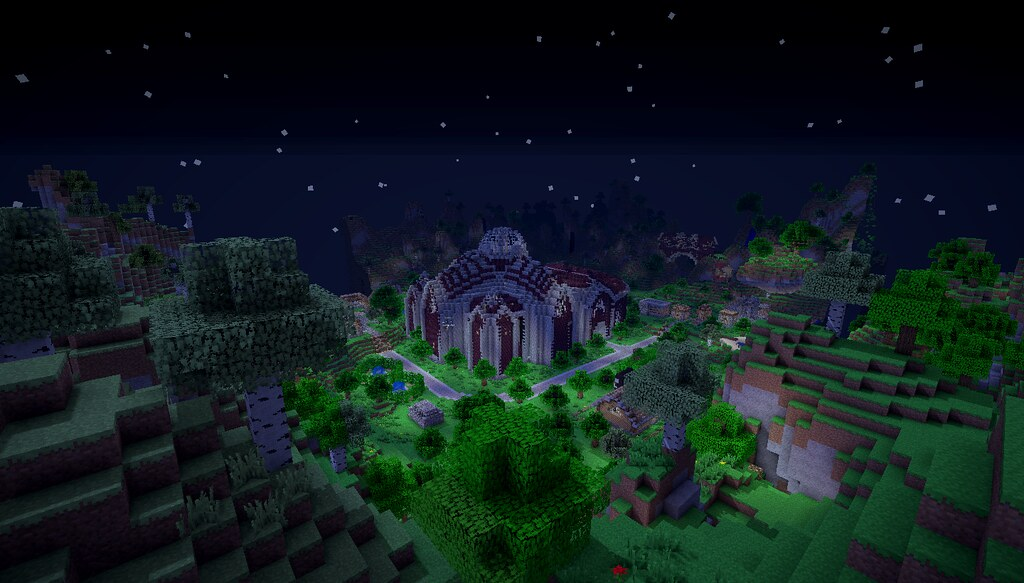
\includegraphics[width=0.75\textwidth]{media/media/image2.jpg} 
    \caption{Example Minecraft world \\ (\href{https://live.staticflickr.com/8167/7659790494_78158cf095_b.jpg}{{https://live.staticflickr.com/8167/7659790494\_78158cf095\_b.jpg}}). CC BY-NC 2.0} 
    \label{fig:2_4_1} 
\end{figure}

\subsubsection{Custom Minecraft Servers}

Minecraft servers have evolved throughout the years, starting from
simple survival servers with small extra features to game modes which
look and feel like a new game completely. Minecraft itself comes with
goals for the player to accomplish in the form of Advancements (a type
of achievement), and custom servers often focus on changing the goals of
the game. For example, a custom server might remove the
resource-gathering aspect of the game to focus on player versus player
(PvP) content.

Custom Minecraft servers have become incredibly popular in the past few
years. The most well-known of these servers, Hypixel, hosts nearly
twenty custom game modes. The server reaches nearly 100,000 concurrent
players during peak hours of the day \parencite{minecraftservers}, making
it the most popular independently managed game server of all time
\parencite{guinnessindependentserver}. While there is no public data on the
company's income, it has been estimated that Hypixel makes between five
million and ten million dollars per year based on employee salary and
number of employees. The custom game modes featured on the server
include "Bedwars", a game where players team up to protect their bed
while attempting to destroy the other teams' beds at the same time. This
game mode adds new mechanics to Minecraft for gathering resources and
fighting opponents. Figure 2.4.1.1 shows a Bedwars game in progress.
Some of the modified elements include the scoreboard on the right side
and health and team display above each player. Another game mode, "UHC
Champions", spawns players in a limited Minecraft world where they must
gather resources to fight each other, but there is a twist. Players can
only regain health through hard-to-acquire "Golden Apples", and the last
remaining player wins. This game mode features custom items added to the
game such as an axe which strikes lightning when attacking other players
\parencite{hypixelgames}.

\begin{figure}[h] 
    \centering
    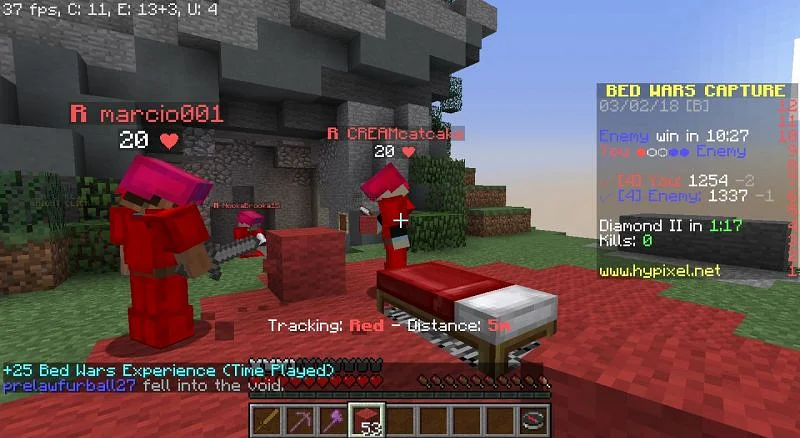
\includegraphics[width=0.75\textwidth]{media/media/image5.png} 
    \caption{Bedwars game in progress, Hypixel, 2021 \\ (\url{https://www.sportskeeda.com/minecraft/top-5-things-players-know-bedwars-minecraft}).
} 
    \label{fig:2_4_1_1} 
\end{figure}
%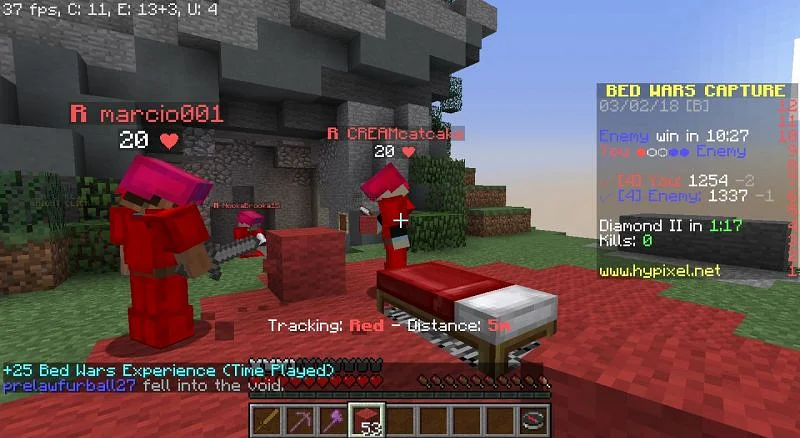
\includegraphics[width=5.60938in,height=3.06538in]{media/media/image5.png}

%Figure 2.4.1.1: Bedwars game in progress, Hypixel, 2021
%(\url{https://www.sportskeeda.com/minecraft/top-5-things-players-know-bedwars-minecraft}).

While Hypixel features significant modification to the Minecraft server,
the gameplay remains similar to the original game. Other popular servers
take a more extreme approach to creating new experiences. One such
example is Origin Realms. Using only server-side modification, Origin
Realms creates an experience which feels like a completely different
game while still maintaining the same core gameplay. The server adds new
blocks, items, creatures, and complete biomes to the game. An example of
the server can be seen in Figure \ref{fig:2_4_1_2}, which shows a completely
custom creature added to the game. These extreme modifications are done
through a combination of server software modification and the Minecraft
resource pack system. Resource packs allow ``players to customize
textures, models, music, sounds, languages, texts such
as the end poem, splashes, credits, and fonts without any code modification'' \parencite{resourcepack}. 
They can be installed on the client, or sent to the client automatically when joining a server.
Using resource packs, custom models such as the turkey in Figure \ref{fig:2_4_1_2} can be loaded by the client and moved or animated by the server.

\begin{figure}[h] 
    \centering
    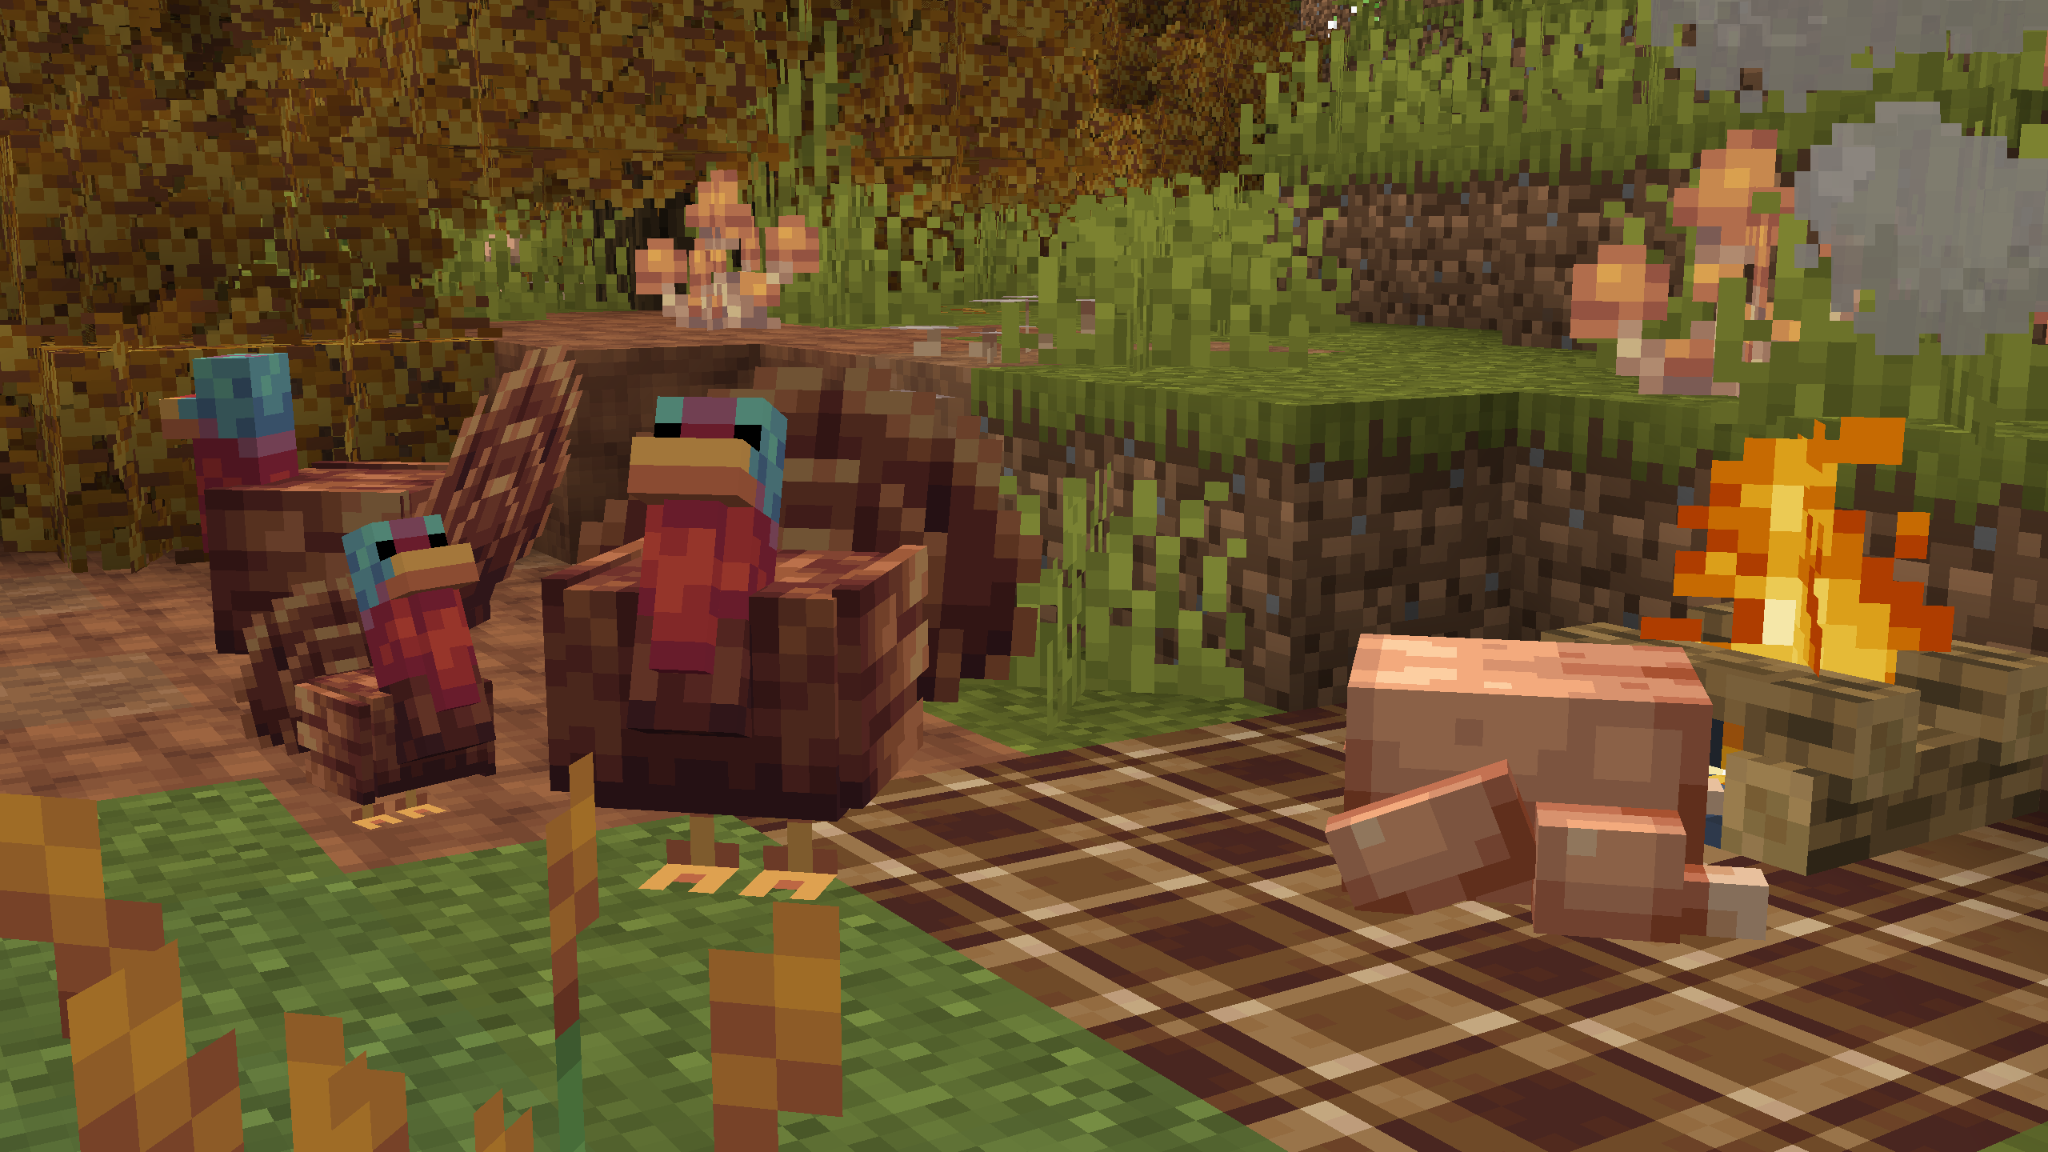
\includegraphics[width=0.75\textwidth]{media/media/image4.png} 
    \caption{Custom turkey creature added to Minecraft, by Origin
    Realms, 2022 \\ (\url{https://originrealms.com/blog/harvesting-update}). }
    \label{fig:2_4_1_2} 
\end{figure}

\subsection{Minestom}

Started in July 2019 by TheMode, Minestom aims to reimplement the
Minecraft protocol from scratch in Java. Most custom Minecraft servers
are created using a modified version of the server published by Mojang,
whereas Minestom was started from scratch. This methodology comes with
some tradeoffs. When modifying the Mojang server, all of the game
features such as entity behavior, block interactions, and much more are
already implemented. Minestom, on the other hand, requires the developer
to implement all of these features if a server wishes to use them. As
such, it makes the most sense to use Minestom when ``removing the
features you don't need takes more time than implementing the ones you
do'' (Minestom Contributors, personal communication, 2022). Using
Minestom does not only come with disadvantages, however. Mojang's
Minecraft server has been in development since the game's release more
than 10 years ago, and it contains a huge amount of legacy code which
could be optimized significantly. Minestom, on the other hand, was
created with a focus on performance, and it does just that. As of April
2021, it can easily handle more than 1,000 players in a basic
environment \parencite{minestom1500players}.
Since then, internal benchmarks have shown
Minestom's capability to handle more than 5,000 players at once
(Minestom Contributors, personal communication, 2022). Additionally,
Minestom allows the programmer to work at a packet level to implement
features very easily, whereas frameworks such as Spigot require the
programmer to work with an unstable API based on deobfuscated code.

\subsection{Past Work}

Test-driven development has become a popular technique in recent years,
and as such this project is not the first to attempt to bring testing
into the Minecraft world. Relevant past works include Mojang's GameTest
framework, MockBukkit, McTester, and a prototype internal Minestom
testing tool. Unfortunately, none of these solutions meets the needs of
high level testing in the Minestom ecosystem.

\subsubsection{Mojang GameTest}

Mojang itself has created two similarly named tools for testing both the
Java and Bedrock Editions of Minecraft. Both tools are named GameTest,
so they will be referred to as Java GameTest and Bedrock GameTest for
the purpose of this report. Java GameTest is completely internal,
whereas Bedrock GameTest was made available to the public in June, 2021
\parencite{ammerlaan2021}. Both frameworks operate on the premise that a
developer can create a structure inside the game, and write some code to
operate on the structure as well as make assertions. Listing 2.6.1.1
shows a sample test from the Bedrock GameTest framework. As seen on
lines 14-16, a test is registered with a structure to contain the test,
and a function to set up the initial state and make assertions. The
example test requires that the victim--a fox in this case--is in the
test area when it starts (Line 8) and not when it ends (Lines 9-11).

```js

// Listing 2.6.1.1

// Adapted from
https://docs.microsoft.com/en-us/minecraft/creator/documents/gametestbuildyourfirstgametest

function simpleMobTest(test) \{

const attackerId = "fox";

const victimId = "chicken";

test.spawn(attackerId, new BlockLocation(5, 2, 5));

test.spawn(victimId, new BlockLocation(2, 2, 2));

test.assertEntityPresentInArea(victimId, true);

test.succeedWhen(() =\textgreater{} \{

test.assertEntityPresentInArea(victimId, false);

\});

\};

GameTest.register("StarterTests", "simpleMobTest", simpleMobTest)

.maxTicks(410)

.structureName("startertests:mediumglass");

```

The Java version of GameTest behaves in a similar manner; however, it
uses Java for test functions instead of JavaScript. According to \textcite{knilberg2020}, a member of the Java gameplay team at Mojang, the test
framework has a few central goals. Tests must be easy to read, write,
and run, they must run visibly in an actual Minecraft world as well as
on a build server, and they must be quiet on success but verbose on
failure. Figure 2.6.1.2 shows some examples of what the tests look like.
Individual test cases are inside the white bounding boxes, and a concise
output is sent to the player when tests pass. This model serves as a
great inspiration for creating and running tests inside the game, but it
has significant flaws for widespread use. It is not made for Minestom
and therefore makes a number of assumptions about Mojang features being
implemented. Furthermore, the framework is closed source, so
modifications are challenging, ineffective in a different environment,
and cannot be distributed.

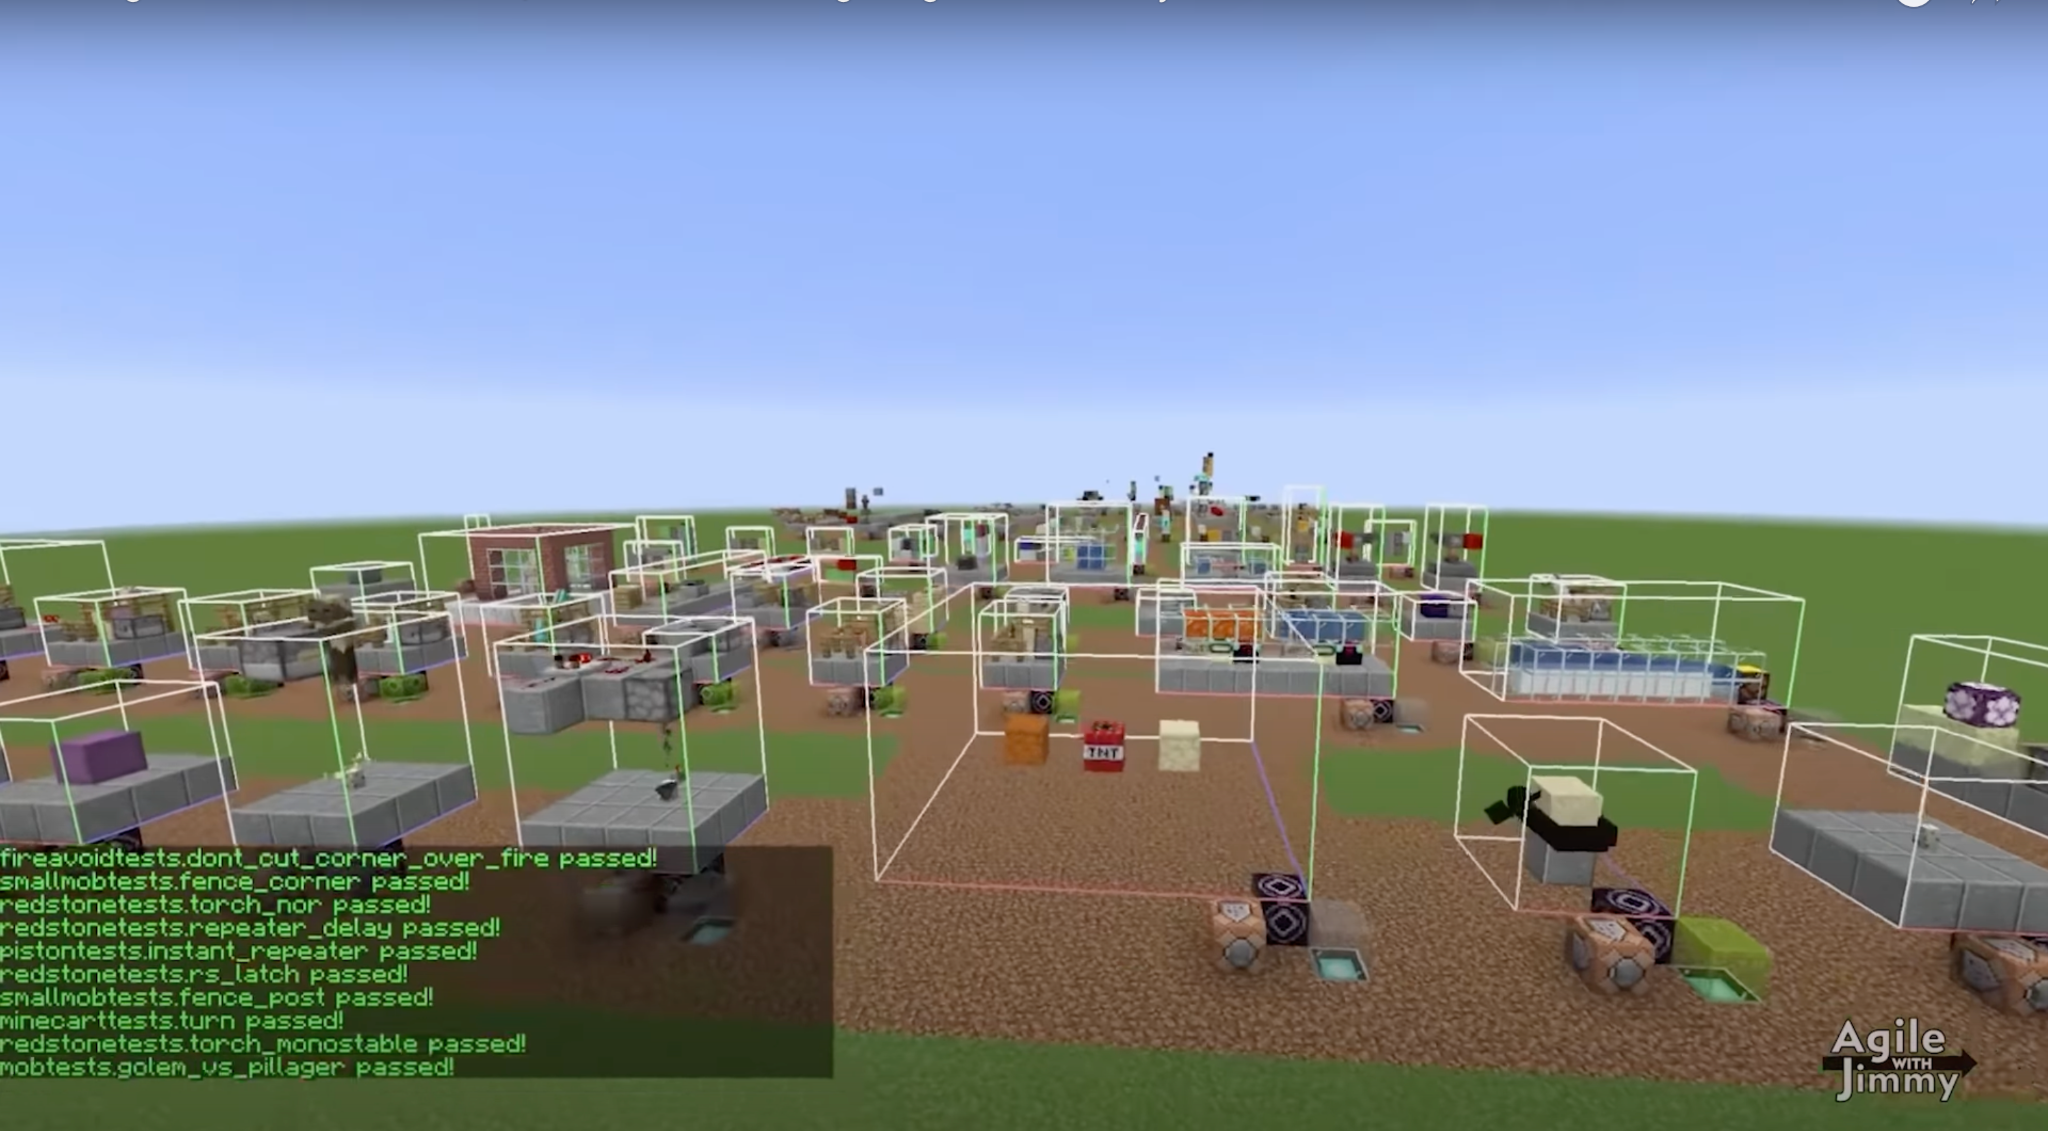
\includegraphics[width=6.01042in,height=3.20833in]{media/media/image7.png}

Figure 2.6.1.2: Example tests from the Mojang (Java) GameTest framework

\subsubsection{Third Party Tools}

In the category of modifications to the Mojang server, there have been
two major attempts at automated testing: MockBukkit and McTester. Both
take a programmatic approach to testing and target different use cases.
MockBukkit provides the user with an API for creating mocked resources
such as players, worlds, and Bukkit plugins \parencite{mockbukkit}. 
This approach allows for a variety of testing methods; however, since the
tests are created programmatically, even simple tests are time consuming
to write. McTester works by running a modified Minecraft client which
allows the test code to submit commands to the client. The server can
then make assertions about the result of the client actions server side.
For example, a test could include a client right-clicking a Command
Block and asserting that the GUI was only opened if the player had
appropriate permission \parencite{mctester}. 
This method of end-to-end testing is effective for testing a server implementation, such as testing
Minestom internally. Unfortunately, it introduces unnecessary overhead
for testing applications built on top of Minestom. Applications
generally do not interact with the client directly, and the actual
server internals are expected to be tested and working independently.
Finally, Minestom has seen its own attempt to create a testing framework
internally. This framework involved a mocked client connection to the
server, from which a test could submit packets and make assertions on
the received packets. Similar to McTester, this can be effective for
testing internal features; however, it becomes cumbersome to work on a
packet level when testing user created features.

\section{Requirements}

As previously discussed, this project aims to fill a void in the
Minestom ecosystem for testing solutions. We hope to create a library to
be the de facto standard for end-to-end testing in the Minestom
ecosystem. In order to meet this goal, we need to consider two main
factors: ease of use and coverage of major use cases. Ease of use means
that developers using Canary should not feel like they have to fight
with the library in order to accomplish what they want. The library
should be internally consistent and predictable, while handling the
needs of developers. To cover major use cases, Canary should be
applicable to the scenarios where developers would want to write
end-to-end tests.

To figure out what standard usage might look like, we looked towards the
greater Minecraft server modding community to see what sort of features
or functionality people have implemented within a Minecraft server.
Although the functionality and features that people add to Minecraft
servers are broad and diverse, we can break them down into a few general
categories based on what they require from a testing library. Depending
on how a feature affects the world, it may require different approaches
for testing. We will look at three broad categories of functionality
that can be added to a Minecraft server.

\subsection{Custom Entity or Block Behavior}

This category refers to most world behavior that is not linked to the
player. This includes entity AI, entity properties, block properties,
how blocks interact with other blocks, and more. Generally these
features only affect a small area around the block or entity, and they
happen based on the state of the world and not the actions of players in
the world. Manually testing these types of features would generally
involve building some sort of setup that will cause the desired behavior
to occur and then watching for the behavior to happen as expected. For
example, to test that minecarts roll down hills correctly, the developer
would first build a track down a hill and then place a minecart on that
track. Then they would watch for the minecart to end up at the bottom of
the track. Canary allows developers to define the setup (structure) for
a test, as well as the expected outcome, and then execute the test on
its own. The required functionality is as follows:

\begin{itemize}
\item
  Define the starting state of a test, including the blocks, block
  properties, and entities.
\item
  Check if expected outcomes happened.
\item
  Run the test until it passes or fail if it has not passed during a set
  lifetime.
\end{itemize}

Determining if the expected outcome happened, in general, is a
challenging problem. There are a wide variety of things that someone
might look for to determine if a test ran correctly. Examples include
looking for an entity to get to a location, looking for a block to be in
a certain state, making sure some condition did not happen, or checking
for things to happen in a certain order. Section 4.2 discusses
assertions more in-depth.

This category of feature benefits the most from end-to-end testing.
Because most of the behaviors only cause changes in a small area, tests
can be run simultaneously without having to reset the entire world
between tests. On top of the functionality requirements, the process of
making, running, and debugging these tests should be simple and
straightforward to align with the overall goal of ease of use.

\subsection{Custom Server Commands}

Server commands are a way to use player messages like a command line or
terminal. Custom commands are a common way to implement features like
switching between worlds, interacting with server mods, or configuring
settings. Server commands, unlike entity and block behavior, frequently
affect things far beyond the player, including internal server state. To
test server commands we should be able to do the following:

\begin{itemize}
\item
  Execute a command from a simulated player with a known starting state.
\item
  Check for the expected behavior of the command.
\end{itemize}

Server commands present a particular challenge because their behavior is
not bound in any way. A server command can do anything from changing a
block near the player, to teleporting the player, to affecting other
players, worlds, or even the entire server. This broad scope makes it
challenging to be able to effectively test all varieties of server
commands, because creating a known starting state could require
restarting the entire server between every test, which would seriously
impact the ability to quickly run tests.

\subsection{Customizing Player Interaction}

If a Minecraft server is aiming to alter the player experience, they
will likely have to change how the player interacts with different
aspects of the world. These changes could be anything from teleporting
the player when they click on an item in their inventory to altering the
world based on how many enemies the player has killed. Custom player
interactions, like server commands, can affect all aspects of the world
and the players in it. Enabling developers to test player interactions
requires the following:

\begin{itemize}
\item
  Simulate a player from a known starting state in a known context
  interacting with the world in some particular way.
\item
  Check for the expected behavior of the interaction.
\end{itemize}

Player interaction often causes changes that can be challenging to test.
The changes may interfere with other tests, or require careful setup and
teardown to ensure the test succeeds when run multiple times. That being
said, some types of player interaction, such as combat or how players
interact with blocks, may be easier and more straightforward to test.

\subsection{Final Requirements}

There are many challenges to creating a test framework that covers all
expected use cases. Features such as server commands and custom player
interaction can potentially change the server in ways that affect the
outcome of other tests. Being able to test every possible feature in a
consistent and reliable manner would require restarting the server
between every test. This would substantially slow down running tests as
well as make it harder to see and debug failing tests, forcing the
library to be much less useful overall. For this reason, we chose to
focus mainly on testing custom entity and block behavior features which
can be tested in a confined area. These features can require elaborate
setups to fully test, and stand to benefit the most from automated
end-to-end testing. That being said, we have not entirely ignored other
feature types, and they could be the focus of future work. From this, we
can create a list of the high level requirements of Canary. We have
split the requirements into two categories, based on our original goals
of ease of use and full feature coverage.

\textbf{Ease of Use}

\begin{itemize}
\item
  Canary must be easy for developers to use, including creating,
  running, and debugging tests.
\item
  Allow developers to create tests in a way similar to how they would
  when manually testing.
\item
  The code API used when writing code for tests should be understandable
  and abstract away common operations
\item
  Silent on success, verbose on failure.
\item
  Tests should be fast to run on a local machine
\item
  Tests should run on Continuous Integration/Continuous Development
  (CI/CD) servers.
\item
  Integrate nicely with version control.
\end{itemize}

\textbf{Feature Coverage}

\begin{itemize}
\item
  Canary must be applicable to all major use cases; in particular,
  custom block and entity behavior should be able to be tested by
  Canary.
\item
  Developers should be able to express complex scenarios in their tests.
\item
  Cover most common usage and allow for easy developer extension.
\end{itemize}

\section{Implementation}

With the high level requirements determined, they must be translated
into specific requirements to be implemented in software. The approach
takes inspiration from the Mojang Java GameTest framework. The key
concept from this work is the combination of a simple structure and code
to create assertions for the test. This approach allows for the creation
of tests to be done largely inside Minecraft, the same way that someone
would when manually testing. Additionally, it reduces the amount of code
required for each test, further improving ease of use. The
implementation of this system can be split into three broad categories:
the test builder, assertion engine, and test executor.

\subsection{Test Builder}

As discussed, Canary tests have a test structure associated with them.
The structure is not defined by code, it is data that is loaded from the
filesystem into the world when a test is being run. To make Canary easy
to use for developers, we allow them to create these structures in the
same way that they would when manually testing: by building them in
Minecraft. The test builder is the subsystem of Canary responsible for
letting users create and manipulate these structures. It allows users to
build structures in game that will then be saved in a form that can be
ingested when running tests.

The test builder allows for the creation of all the necessary starting
conditions for tests. It is easy to use and has convenience features
that users frequently need when creating end-to-end tests, such as
basing the structure for one test off of the structure of another. The
created structures allow users to edit the properties of the blocks,
either to change how they behave or to mark them so their position can
be referenced from the code associated with the test (mark a block with
a name that can be used to easily get the position of the block).
Because the test builder runs on the server, it has multiplayer support.
This means that multiple players can work on a single test structure at
once and that different players can work on different structures
simulatniously.

Once a user has built a test structure, it is saved in a format that can
be loaded into the world when running tests. For git compatability,
structure files are text-based so that minor changes to the structure
will not cause git to see the whole file as changed.

When using the test builder, a player is brought into a separate empty
world containing just the structure they are creating or editing (Figure
4.1.1). The advantage of this approach is that it becomes simple to
track all of the blocks that are part of the structure, and there is no
risk of other parts of the world interfering with creating the
structure.

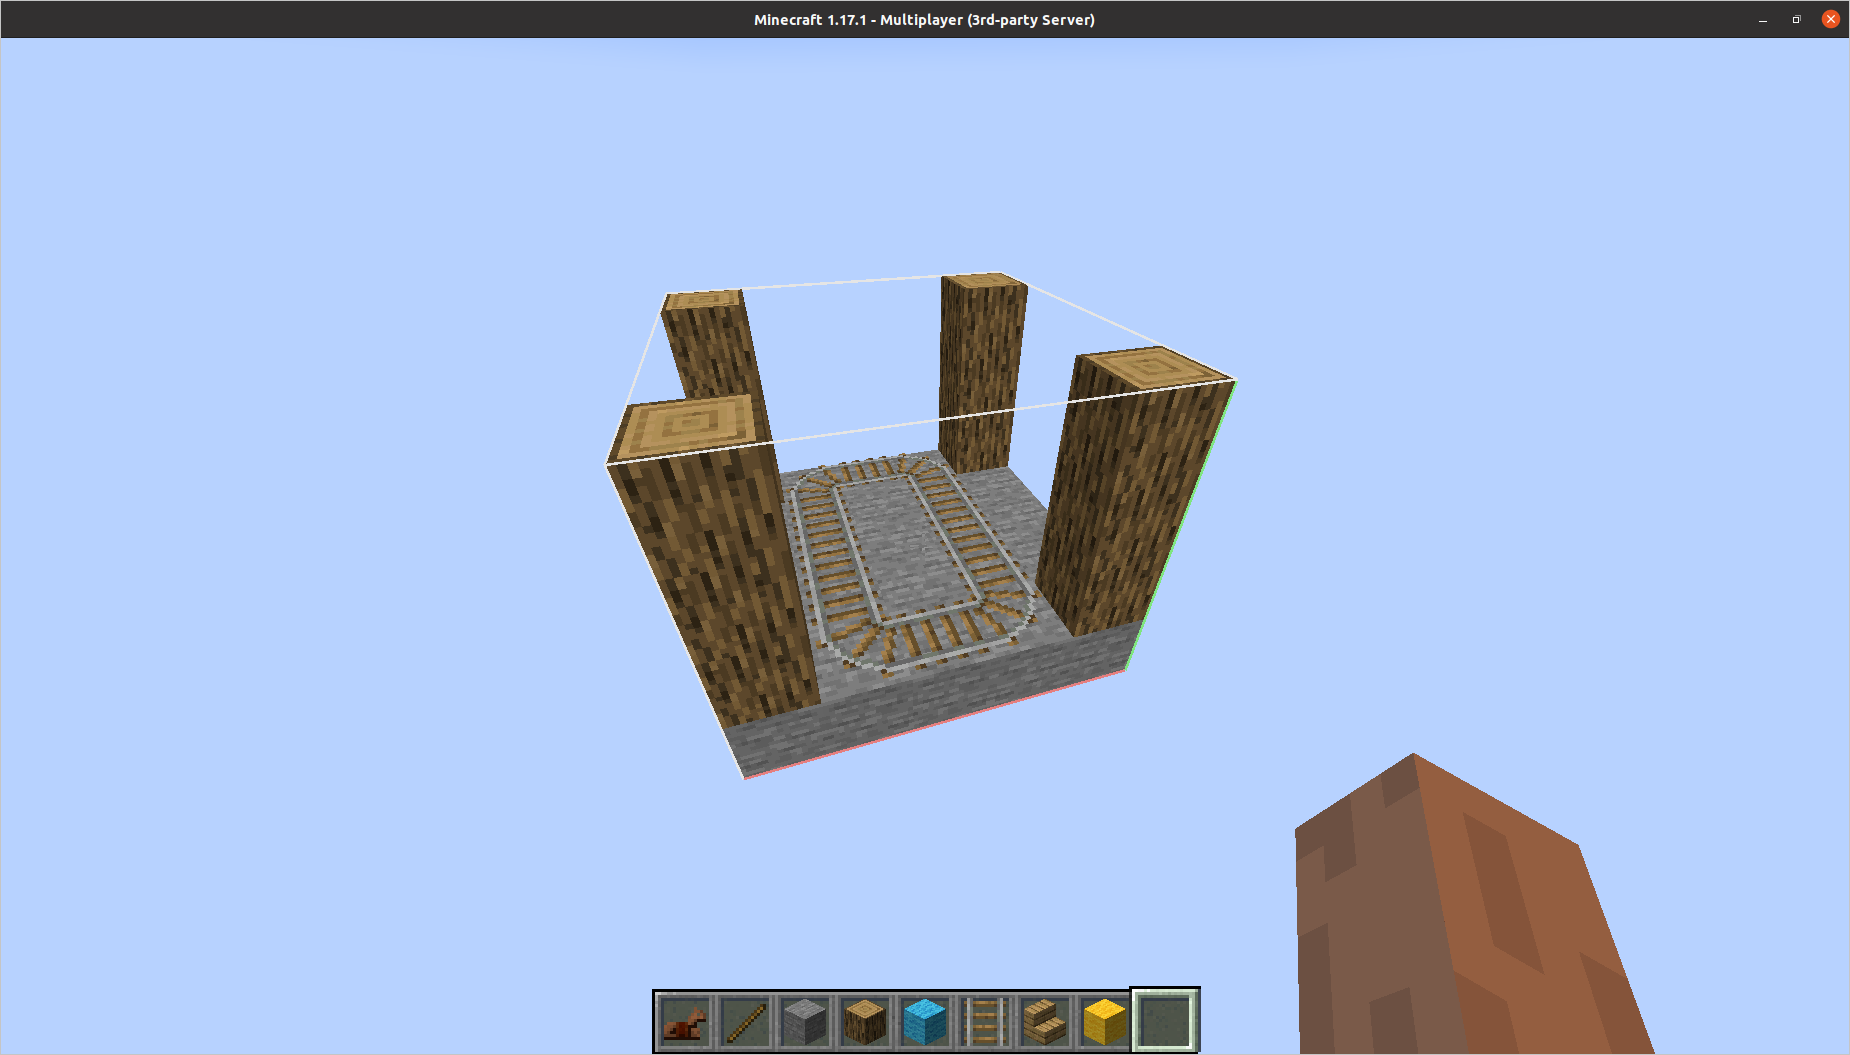
\includegraphics[width=6.5in,height=3.56548in]{media/media/image9.png}

Figure 4.1.1: Example of a structure in the test builder

The way that the player controls the test builder--including making a
new structure or leaving the test builder when they are done creating
their structure--is through server commands. Server commands are a
feature of Minecraft that are similar to a command line. Using the
in-game chat, messages starting with a forward slash are considered
commands. Minecraft and Minestom have powerful support for commands,
including named arguments and autocomplete. As seen in Figure 4.1.2,
Canary can suggest possible valid inputs when they are known.

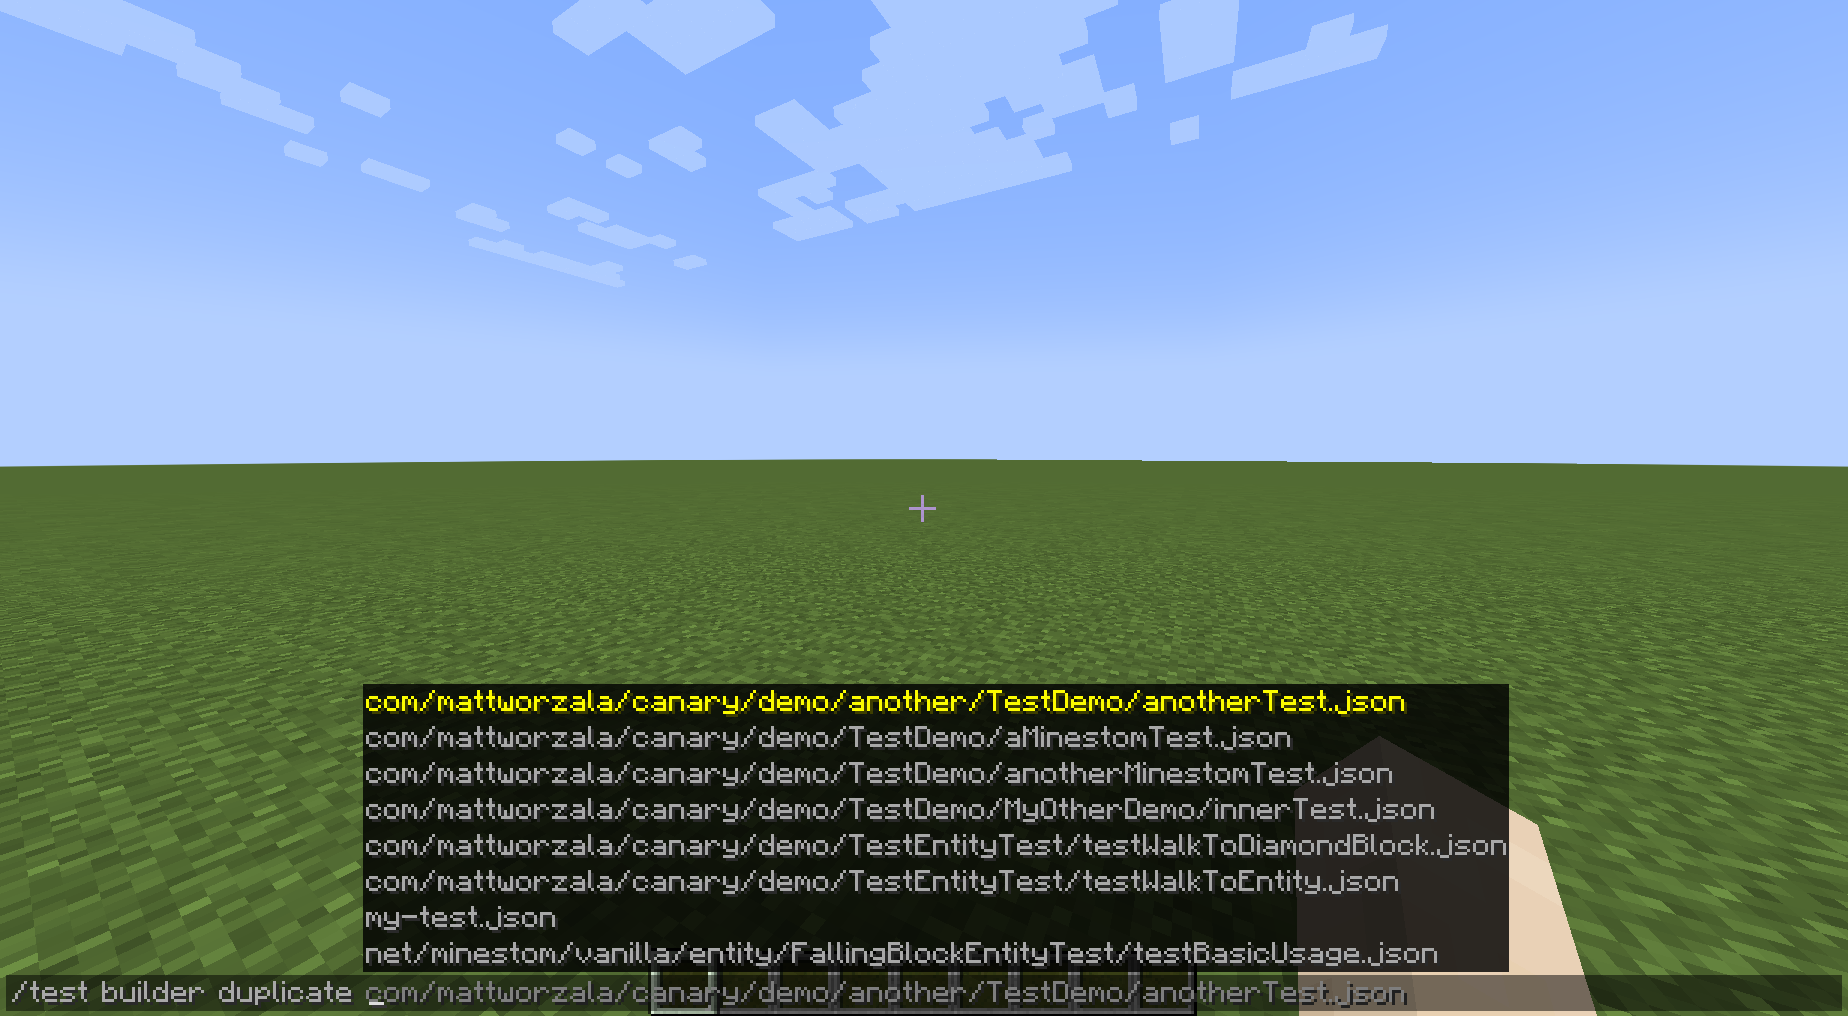
\includegraphics[width=6.0625in,height=3.32292in]{media/media/image13.png}

Figure 4.1.2: Autocompletion of existing test structure when using the
duplicate command.

The test builder commands available to the player change depending on
whether or not they are currently in the test builder. When the player
is not in the test builder, the commands available to them are as
follows:

\code{/test builder new STRUCTURE\_NAME}

Places the player in a test builder world with the default starting
structure. When they save the structure, the file will be named
\code{STRUCTURE\_NAME.json}.

\code{/test builder duplicate STRUCTURE\_NAME NEW\_STURCTURE\_NAME}

Places the player in a test builder world with structure from
\code{STRUCTURE\_NAME.json}. When they save the structure, the fill will be
named \code{NEW\_STRUCTURE\_NAME.json}.

\code{/test builder join CURRENT\_STRUCTURE\_NAME}

When there is a player currently building a test, this command is how
you join them in the test builder.

When the player is in the test builder, the commands available to them
are as follows:

\code{/test builder done}

Saves the current structure and returns the player to wherever they were
when they entered the test builder.

While in the test builder, players can freely place and remove blocks.
The creative mode of Minecraft gives players the ability to place any
block in the game by choosing it from a list. To help users visualize
the structure that they are building, a white bounding box is placed
around all of the blocks that are a part of the structure. This box is
updated as players place and remove blocks to always bound the entire
structure. This is accomplished using a Minecraft structure block. A
structure block is normally used during world generation in vanilla
Minecraft, but for our purposes the white bounding box is all we need
(Figure 4.1.3). A structure block is placed below the build area, and
its parameters are updated as necessary to change the size and position
of the bounding box that it creates.

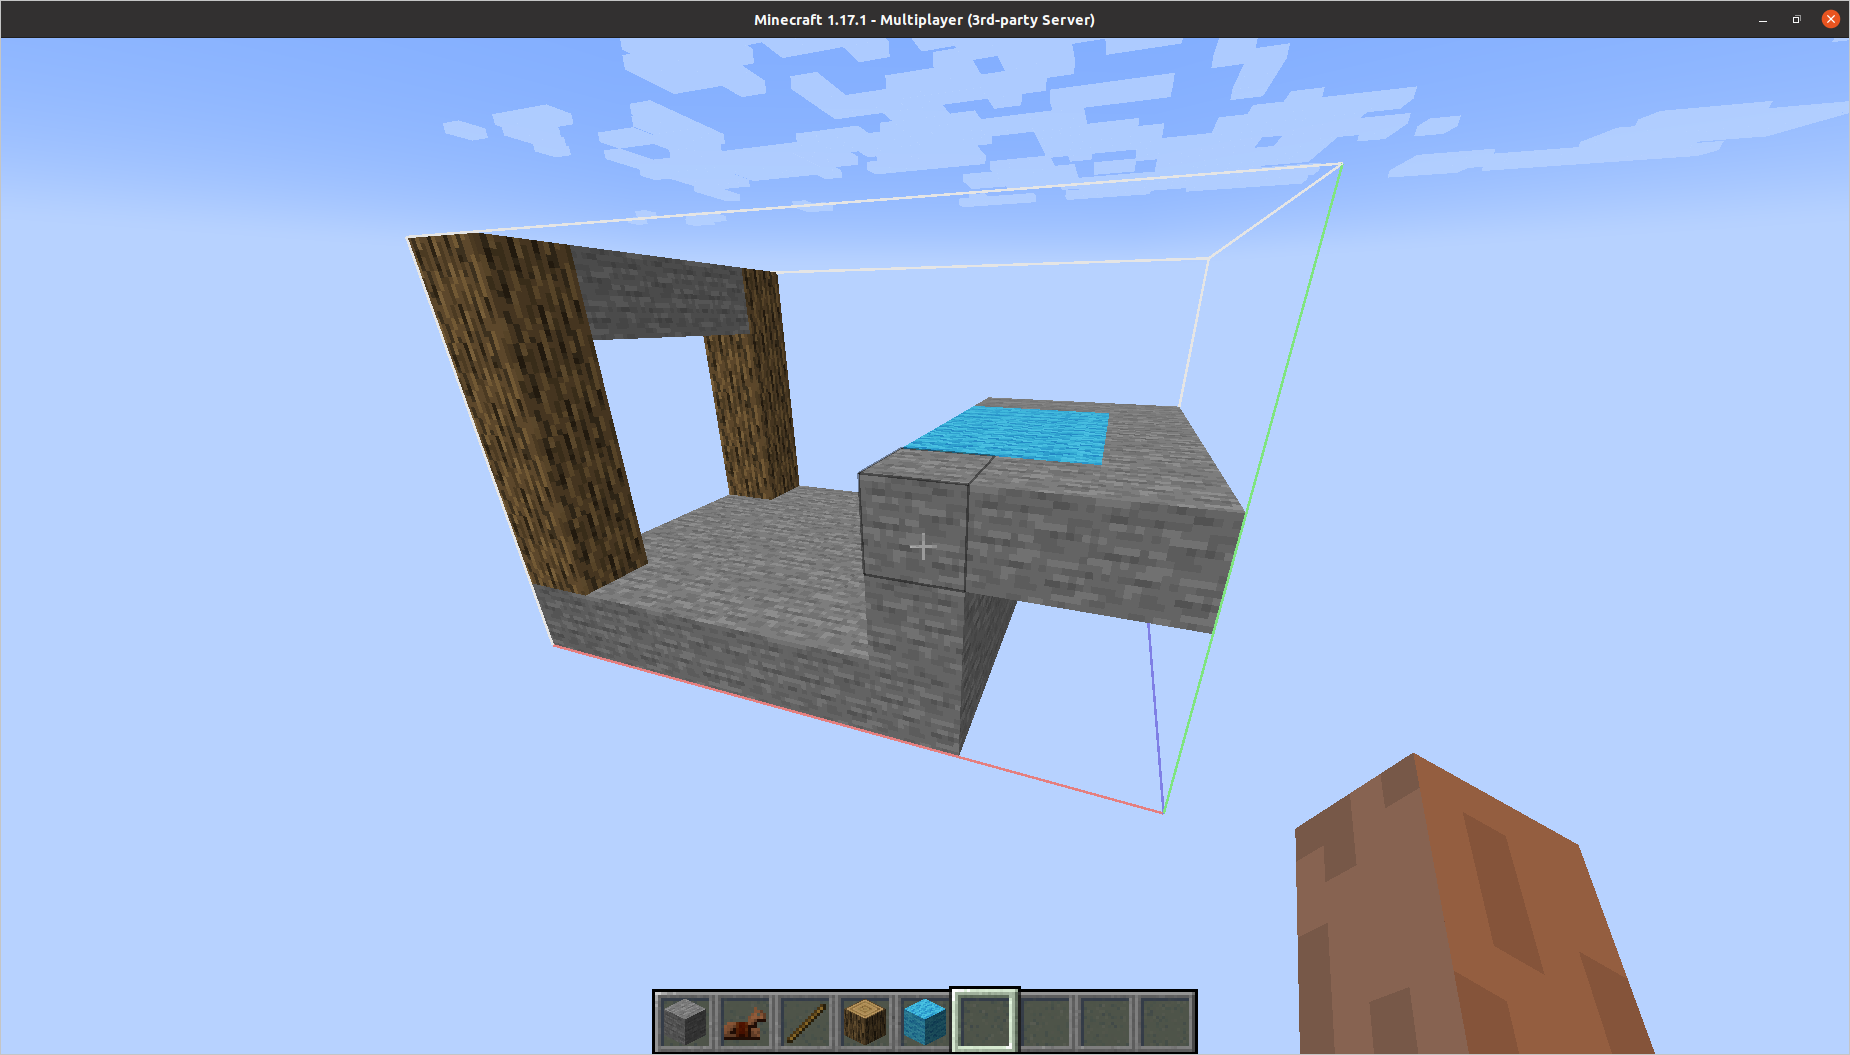
\includegraphics[width=6.07813in,height=3.34897in]{media/media/image11.png}

Figure 4.1.3: The bounding box tracks the size of the structure

The other important functionalities within the test builder are editing
the properties of blocks and placing markers. Blocks have data
associated with them beyond just what type of block they are. This
includes information like the orientation of the block, what Java class
is responsible for handling the block's behavior, and many other
properties. The fields cannot normally be set in Minecraft; they
generally are set by the game itself. Markers are a concept introduced
by Canary as a way for a user to give a name to a position within the
test structure. The marker name can be used to get the location of the
marker in the code for a test. Markers allow for a more ergonomic
alternative to putting raw coordinates in a test.

These two functionalities were implemented using the same general
principle, which is to give the player items with special behavior when
used to click on an item. While Minecraft does not have a built-in
method to prompt the user for typed input, there are multiple different
methods that can be implemented to approximate the desired behavior. Two
such examples are using the in-game chat and making use of the anvil
inventory screen, which has a box for text entry. Using these, we can
prompt the user to enter information when they click on a block with one
of the special test builder items. For example, with the set marker
item, after clicking on the block they want to mark, the user will be
given an anvil prompt (Figure 4.1.4) where they can enter the desired
marker name. Then they can click on an item (green glass) used as the
confirm button or another item (red glass) used for canceling. This will
then create a marker with that name at that location in the test
structure. A similar process can be used for the various types of block
data.

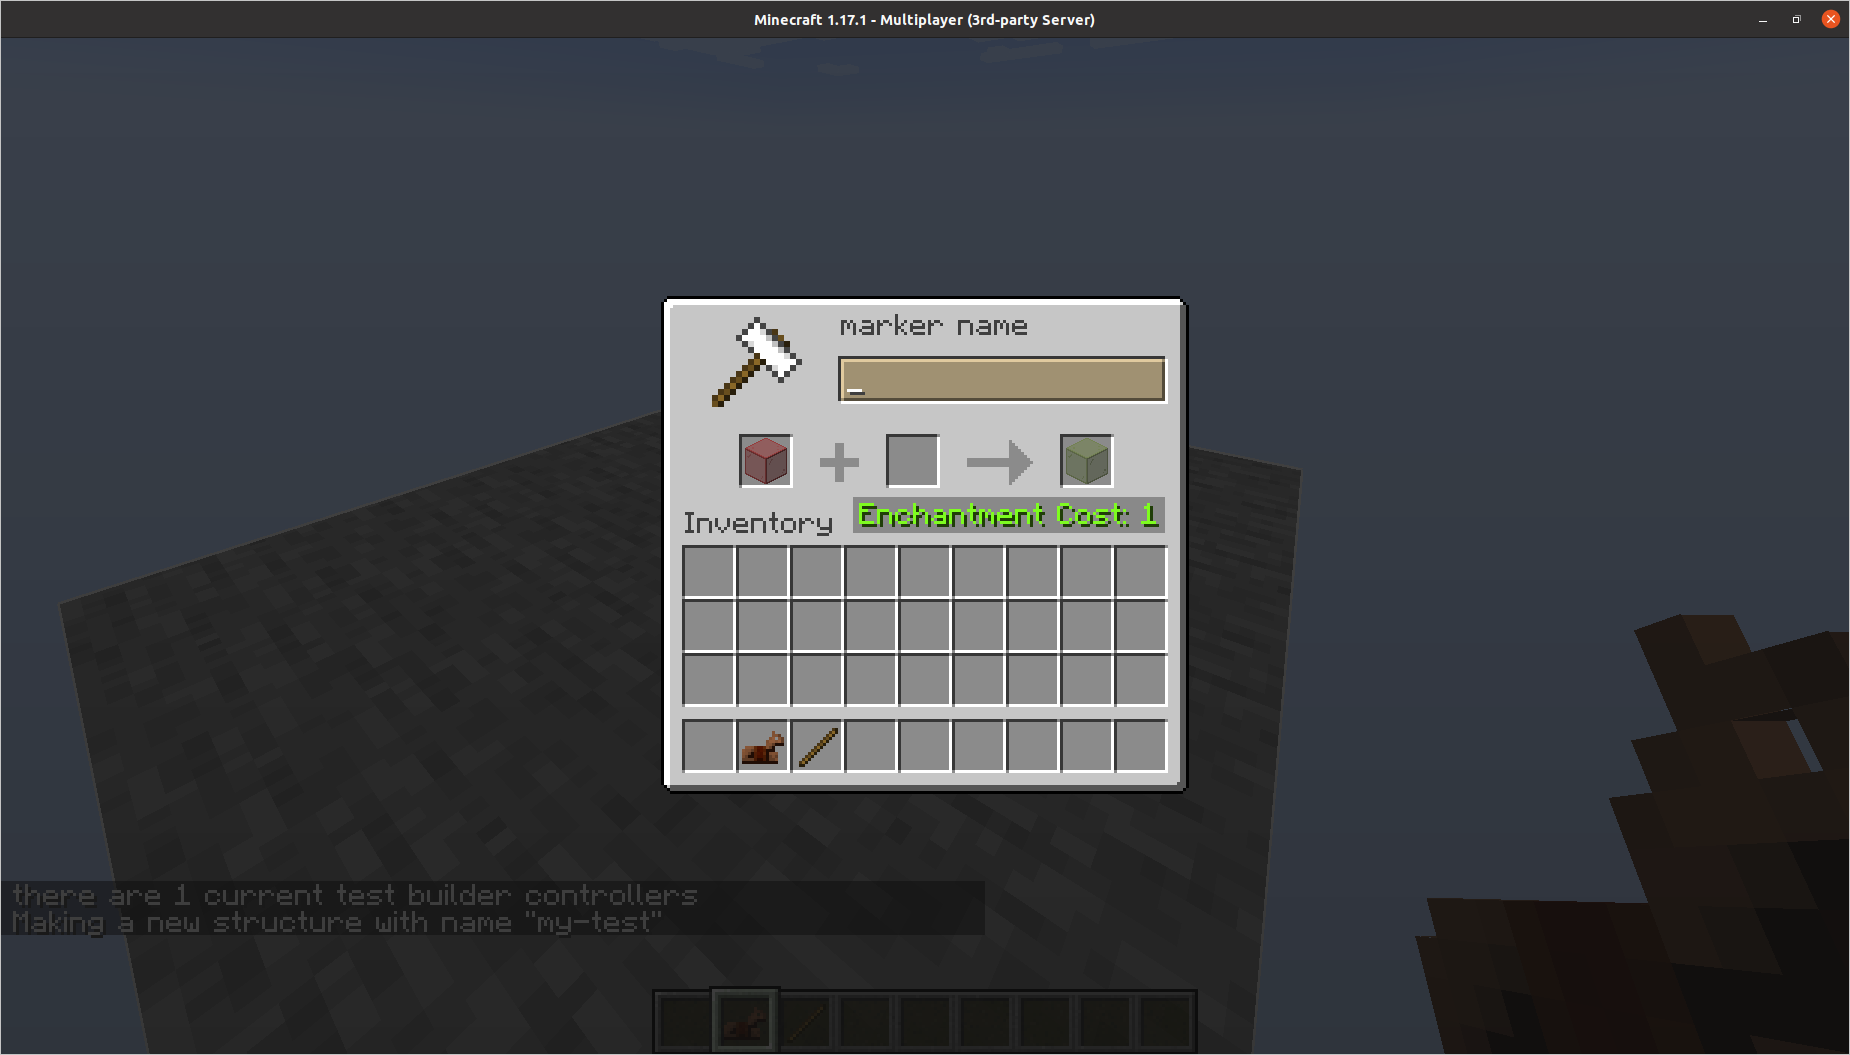
\includegraphics[width=6.16146in,height=3.3967in]{media/media/image8.png}

Figure 4.1.4: Example of the anvil prompt for markers

Behind the scenes, all of these special items pass the position of the
block that was clicked on--along with the data the user entered--to
commands that are part of the test builder. These commands can also be
used instead of items if desired by a user. The two commands currently
implemented by Canary are for setting a marker and setting the block
handler property of a block. They are defined as follows:

\code{/test builder edit marker X Y Z MARKER\_NAME}

Creates a marker at position (X, Y, Z) with the given name.

\code{/test builder edit handler X Y Z HANDLER\_NAME}

Sets the block handler for the block at position (X, Y, Z) to be the one
defined by the given name.

\subsubsection{Structure Files}

As previously mentioned, the test structures created using the test
builder are saved using a text format, specifically a JavaScript Object
Notation (JSON) file. This format was chosen because it is both human
and machine readable, and is reasonably compact. The fields within the
file use a format custom to Canary that was created to be easy to create
and parse while trying to minimize the size of test structure files.
Large software projects can have hundreds or even thousands of tests,
and an overly verbose format could cause test structures to use up an
unnecessary amount of disk space. Listing TB.1 shows a sample test
structure file.

```json

// Listing TB.1

\{

"id": "my-test-world",

"size": {[}

16,

16,

16

{]},

"markers": \{

"diamond\_block": 123

\},

"blockmap": {[}

"minecraft:stone",

"minecraft:cobblestone\_stairs{[}facing=north{]}",

\{

"block": "minecraft:stone\_stairs{[}facing=south,waterlogged=true{]}",

"handler": "example:my\_block\_handler",

"data":
"\{name1:123,name2:\textbackslash"sometext1\textbackslash",name3:\{subname1:456,subname2:\textbackslash"sometext2\textbackslash"\}\}"

\}

{]},

"blocks": "0,256;1,16;0,240;-1,3584"

\}

```

The fields of the JSON file in Listing TB.1 are specified as such.

\textbf{id}

Some unique id to be referenced from the test code.

\textbf{size}

The x, y, and z size of the structure, with a max of 48, 48, 48.

\textbf{markers}

An object where each key-value pair represents the name and position
index of the marker. The position indexing uses the same scheme as
described for the block's value.

\textbf{blockmap}

An array where each element represents a block which is used in the
structure; a block id of \code{-1} represents a block of air with no additional
properties. A block can have a type, tags, a handler, and additional
data. A block object has a block, handler, and data field. The handler
and data fields correspond directly to the handler and additional data
of the block they represent. The block field represents both the block
type and the block tags as a single string of format
\code{block\_type{[}tag1=tag1\_value,tag2=tag2\_value,...{]}} (if there are
no tags, the square brackets are omitted). If a block has a special
handler or data, it must be defined as using a block object. If a block
just has a type and tags, it can just be stored using a string equal to
what the block string of it's object would be.

\textbf{blocks}

A run length encoding of the blocks for the test. The semicolons
separate each block definition. A block definition starts with a block
id reference the blockmap array, followed by a number of blocks. Since
the structure is three dimensional, but our block definitions are
linear, we need a way to convert between the two ie. find the x, y, and
z coordinates of the n-th block.

Firstly, we define the position (0, 0, 0) as the first position in the
structure. From one position, the next position can be gotten by
incrementing the x coordinate. If the new x coordinate is greater than
the size of the structure, you set the x to be zero and increment the z
coordinate. Likewise if the z coordinate is greater than the size of the
structure, you set the z to be zero and increment the y coordinate. The
order of positions will generally look like (0, 0, 0), (1, 0, 0), (2, 0,
0), ..., (0, 0, 1), (1, 0, 1), ..., (0, 1, 0), (1, 1, 0), ..., assuming
that the structure is large enough to encapsulate all of these
positions.

The run length encoding used in the blocks field is the primary way that
this format helps to reduce file sizes. Most test structures will likely
contain only a handful of different block types, with a lot of
repetition. The run length encoding--along with the block map
array--means that much of that repetition can be stored succinctly. This
format is not the most optimal way to compress this information, but we
have found it does well enough in most use cases, while being easy to
output and parse.

\subsection{Assertion Engine}

Assertions and their associated Application Programming Interface (API)
are an integral part of Canary and one of the most user-facing elements.
They are how the user encodes all expected functionality for the tested
features of their software. In order to meet the project goals, the API
must be highly flexible while remaining simple for obvious tasks.
Assertions in Canary do not happen in a deterministic manner, and they
may happen at an unknown time from the start of the test. This is
because the Minestom server does not run at an exact rate, so there may
be slight differences in behavior between executions. This creates a
significant challenge for writing assertions which remain simple to
understand. The solution adopted by Canary is to allow the user to
define small programs which dictate the expected state of the test
environment throughout its execution time. The program can be
conceptually split into two distinct segments, roughly modeled after a
typical interpreted programming language: assertions themselves
(syntax), and the backing assertion nodes (AST). The syntax of a typical
assertion in Canary can be found in Listing 4.2.1.

```java

// Listing 4.2.1

expect(myZombie).toBeAt(3, 1, 3).and().toHaveHealth(20.0);

```

The syntax is legible like plain English, e.g. "I expect that my zombie
will be at \code{\textless3,1,3\textgreater{}} and have \code{20} health". In this
report, an assertion may be referenced using the following abstract
representation: \code{EXPECT myZombie.pos=\textless3,1,3\textgreater{} AND
myZombie.health=20.0}, or simply \code{pos=\textless3,1,3\textgreater{} AND
health=20.0} for the general case. When the test containing Listing 4.2.1
is executed, the calls generate a list of steps to the assertion. This
step is analogous to tokenizing an input source in a programming
language. The generated list for this case is shown in Listing 4.2.2.

```

// Listing 4.2.2

SUBJECT = myZombie

STEPS = {[}

subject.pos == \textless3, 1, 3\textgreater,

AND,

subject.health == 20.0,

{]}

```

From the step list, the engine generates a tree of nodes, each of which
has the ability to report whether it passed or failed depending on the
condition (e.g. \code{subject.pos == \textless3,1,3\textgreater}) or the
children. For example, the \code{AND} node has the following simple logic:

1. If any child is a \code{FAIL}, return \code{FAIL}

2. Return \code{PASS}

This system is analogous to an Abstract Syntax Tree (AST) in an
interpreter, and it allows the test executor to simply check the root
node to determine the result of the assertion. The nodes recursively
process until all branches have been evaluated or an early exit has been
reached. The test executor acts on the result of the assertion tree, as
described in Section 4.5.

\subsubsection{Soft Pass}

The assertion engine as described above is effective; however, it is not
perfect. A common assertion tool is the \code{NOT} statement. This allows the
user to invert the statement directly following. For example, \code{NOT
health=20.0} says that it will fail if the subject's health is equal to
\code{20}. By defining what causes an assertion to fail, it becomes difficult
to determine when it has passed. Assertions are executed every server
tick until they return a \code{PASS} (further described in Section 4.5). If,
for example, the subject has a starting health of \code{10}, then on the first
frame this assertion will return \code{PASS} and never be tested again. The
solution to this problem is to introduce a third state to the equation:
\code{SOFT\_PASS}. A soft pass indicates that the condition is currently
passing; however, it could fail in the future, so it must be tested
again. This system allows for statements which cannot produce a final
output. Another use case of this system is the \code{ALWAYS} statement. It says
that the following condition \emph{must} be true for the duration of the
test. The \code{ALWAYS} node can never return a \code{PASS}, because the condition
could still change in the next tick, so instead it returns \code{SOFT\_PASS}.

\subsubsection{Assertion Specification}

In order to create the English-like syntax Canary uses for assertions, a
somewhat complicated inheritance hierarchy is used. Each call to expect
returns an assertion class for the specific object passed in, such as an
\code{EntityAssertion} if a Minestom \code{Entity} is passed in. To reduce code
duplication, assertion classes themselves create an inheritance
hierarchy, meaning it is possible to call \code{ObjectAssertion.toBe(Object)}
on an \code{EntityAssertion}. This works fine in isolation; however, it falls
apart when considering chained assertions such as an \code{AND} statement. Each
assertion function returns itself so that more statements can be chained
together, but control statements are defined on the base assertion
class. Consider the code snippet in Listing 4.2.2.1; the \code{and()} call
returns a \code{BaseAssertion} instance, which does not have \code{toBeOnFire()}.
Java does not have a self type like in some languages, so we must use
recursive generics to accomplish a similar effect. Recursive generics
are generic types which reference themselves. The (abbreviated)
definitions for \code{BaseAssertion} and \code{EntityAssertion} can be seen in
Listing 4.2.2.2. \code{BaseAssertion} requires a generic parameter of some type
inheriting from \code{BaseAssertion}. In \code{EntityAssertion}, we fill this
requirement. As a result, the return type of \code{not()} inside
\code{EntityAssertion} is still \code{EntityAssertion}. While this solution does
accomplish the desired goals, it is an unsafe and generally discouraged
practice because there is no strong validation on what is being set as
the generic parameter. This system is internal to Canary, so these
contracts can still be met to create a usable syntax and stability.

```java

// Listing 4.2.2.1

expect(myEntity).toBeAt(3, 1, 3).and().toBeOnFire()

```

```java

// Listing 4.2.2.2

public class BaseAssertion\textless This extends
BaseAssertion\textless This\textgreater\textgreater{} \{

public This not() \{ ... \}

\}

public class EntityAssertion extends
BaseAssertion\textless EntityAssertion\textgreater{} \{ ... \}

```

\subsubsection{Player Interaction Testing}

Most custom Minecraft servers revolve around player interaction rather
than events which happen passively. Creating fake player events for
tests can be somewhat limiting, given the complex back-and-forth between
the client and server. Manually mimicking client behavior in an accurate
manner would be extremely difficult and error-prone, along with
requiring a lot of effort. Instead, Canary proposes recording player
interactions on a live server and playing them back with a simulated
client during a test case. Instead of spawning an entity, for example, a
tester could spawn a player with a packet stream that was "programmed"
in-game inside the test structure itself. The Canary implementation in
this report contains a prototype of this system via a recording
mechanism. There is, however, more to be done for a complete system.

The recording infrastructure in Canary uses a simple binary file format
(named Canary Packet Record, or CPR). The file format is a short header
followed by a list of the binary protocol data received by the server.
The header contains the file format version, the Minecraft protocol
version, and the starting state of the Player. The Minecraft protocol
version must be stored because packet IDs and format change between
versions, meaning the file must be updated. Each entry in the file
contains the time (since start of recording, in milliseconds) that the
packet occurred, and the packet data itself. A detailed description of
the file format can be found on
\href{https://gist.github.com/mworzala/13abec46e1114bde479cb0c9e7e8d888}{{GitHub}}.
Once loaded, a fake player is created which submits the packets to the
server according to the time they occurred in the CPR file.

The prototype implemented in Canary is far from complete, however.
Playing back a recorded interaction requires the tester to manually load
the recording and create the playback player. This system should be a
simple test environment request, which creates, plays, and cleans up the
playback player. Additionally, there are cases, such as player versus
player (PvP) features, where it would be beneficial to have multiple
players recorded in the same session. For this case, the tester should
be able to play one or more recordings while creating a new one so that
they are able to interact with the existing recording. For example,
hitting it with a sword to ensure that damage is dealt in player versus
player combat. Another issue with the packet recording mechanism is the
initial Player state.

\subsection{Test Executor}

The Canary test executor is responsible for managing the testing
environment and complying with the JUnit test engine specification. When
the engine is invoked, it first discovers every potential test case
(method annotated with \code{@InWorldTest}). Each test is loaded into the
appropriate Java ClassLoader, and a Minestom instance is created. An
"instance" in Minestom is analogous to a Minecraft world and allows the
test to be completely isolated from all others. When the tests are
executed, each test structure is placed into its respective instance,
and the assertion engine parses the step lists (Listing 4.2.2) into
assertion trees. Finally, the test instances are ticked until it
receives a definitive result. The stop conditions for a running test are
as follows:

1. Every assertion has returned a \code{PASS} value (pass)

2. Every remaining assertion returns a \code{SOFT\_PASS} value (pass)

3. The timeout limit has been reached (fail)

The second condition is due to the behavior of \code{SOFT\_PASS}. An assertion
such as \code{ALWAYS} cannot ever know that it has definitively passed, so it
exclusively returns \code{SOFT\_PASS} or \code{FAIL}. When a test times out, 
however, it means that there are no more steps so a \code{SOFT\_PASS} is
equivalent to a \code{PASS}. Because Canary tests run over a long period of time 
and state changes throughout, \code{FAIL} does not indicate a definitive failure.
Instead, it indicates that the test has \emph{not yet passed} but may in
the future. If the time runs out and there are still failing assertions,
then the test is a failure.

\subsubsection{Sandbox Versus Headless Mode}

Canary has a strong focus on ease of use and visual feedback through the
sandbox mode of the test engine. Writing tests inside the environment
they are testing provides the user a huge benefit, including real-time
feedback. The user can enter the game and watch their tests running in
real time, making it extremely simple to determine what is wrong. Canary
facilitates this using the "sandbox instance", a Minestom instance
containing every loaded test. This world allows the user to visibly see
which tests are passing or failing, and the user can fly around in the
virtual space to view them. Visual feedback for the developer, however,
is not the only responsibility of a test engine. Test engines must be
able to execute remotely in a Continuous Integration/Continuous
Development (CI/CD) pipeline. Canary refers to this as "headless"
execution mode, and it differs from the sandbox mode in a few ways. The
running test server is not available to join, and the debug information
is not loaded, including commands and the sandbox instance. To ensure
that all tests remain isolated and predictable, each test is still
loaded into its own instance.

\subsubsection{Test Isolation}

It is critical to create the same exact environment for every execution
of a test both locally on multiple distinct machines or remotely as a
part of a CI/CD pipeline. This task is non-trivial in the Minestom
environment, since a test may access and use arbitrary server data or
interact with arbitrary blocks around the test environment. The most
obvious solution is to use a unique Minestom server for each test which
solves the global state and nearby interaction issues in a simple and
intuitive way. Unfortunately, this solution has significant drawbacks in
terms of speed and usability. Minestom makes use of a global (static in
Java) state for running server information, which means that you cannot
easily have two Minestom servers running at the same time. It is
possible to start a Java Virtual Machine (JVM) subprocess for each test
or load each test into its own ClassLoader. Both results incur a large
initialization overhead and memory increase for each individual test
because every class must be reloaded each time. Regarding usability,
separating each test into its own JVM or ClassLoader means that it is no
longer possible to create the aggregate sandbox instance, destroying the
ease of creating tests. Instead, Canary handles isolation by placing
each individual test (and associated structure) into its own unique
Minestom instance. This allows the sandbox instance to remain by
forwarding actions from each sub instance into the sandbox. This
solution, however, does not impose strict isolation for global server
state. In the end, this compromise was worth the benefit provided by the
sandbox instance. Without strict isolation, users are required to write
code which can be tested in isolation. As a result, the code quality
when using Canary should increase.

\subsubsection{Test Environment}

To achieve the goal of simplicity from a user perspective, Canary
provides a utility for various tasks inside the test environment. This
class, TestEnvironment, provides safe access to the Minestom instance
for common tasks such as spawning entities. In sandbox mode, tests may
be executed multiple times, so they must be cleaned up properly to avoid
creating false positives or negatives from leftover changes to the
environment. To accommodate this, the test environment provides a
tracking interface. A user may register a trackable object, which will
have a cleanup method called whenever the test needs to be reset.
Internally, this mechanism is used to remove any entities which are
spawned during the course of the test execution. The test environment
also provides access to the markers defined inside test structures,
without the user directly interacting with the structure file itself.

\subsubsection{Error Reporting}

In any testing framework, good error reporting is a vital element to
success and ease of use. Canary is no exception, but this presents a
complex situation due to the long-running nature of the tests. In most
testing frameworks, errors are presented as the difference between the
expected and actual result. Canary assertions can be complex and not
necessarily dependent on any single tick of the test. For example,
consider the assertion \code{pos=\textless3,1,3\textgreater{}}. If the subject
never reaches the position \code{\textless3,1,3\textgreater{}} before the time
runs out, then presenting the user with the final position is not
necessarily helpful. For cases such as this, Canary records a log file
every frame containing the output of each assertion. This data can be
hard to parse, so it should not be considered as the first resort.
Headless and sandbox modes provide different environments for errors to
be presented, and these are handled individually in Canary.

In headless mode, the output is going to a terminal, meaning the result
can be somewhat long and must encode all relevant information into text.
In this case, Canary logs the failed assertion tree for the failing tick
into the terminal, along with the complete log. An abbreviated failure
in headless mode can be seen in Figure 4.3.4.1. In a CI/CD pipeline,
users typically do not have access to files produced during execution,
so writing a log file is not helpful. Additionally, headless mode does
not give any visual output of the test, so the log is the only available
information. As such, it is recommended that users instead download the
test and execute it locally for an interactive visual output of the
running test.

```

// Figure 4.3.4.1

Testing complete.

1 test failed.

Error: com.mattworzala.canary.demo.TestEntityTest.testWalkToDiamondBlock
- e\_e9f02b@\textless2, 1, 3\textgreater{}

e\_e9f02b did not reach \textless2, 1, 3\textgreater{}

Complete Log

e\_e9f02b@\textless2, 1, 3\textgreater{}

Step 0 : entity1 was at \textless2, 1, 1\textgreater{}

Step 1 : entity1 was at \textless2, 1, 1\textgreater{}

Step 2 : entity1 was at \textless2, 1, 1\textgreater{}

Step 3 : entity1 was at \textless2, 1, 1\textgreater{}

\ldots{}

```

In sandbox mode, the user can see and interact with the test output.
This allows the user to debug the test in the same way as someone might
do when manually testing a feature. In addition, sandbox mode provides
only the last tick failure to the player, deferring to the longer log
file for the complete output of the test. A sample failure report
generated by the sandbox mode can be seen in Figure 4.3.4.2. The message
contains a clickable element (\code{{[}LOG{]}}) to open the log file locally,
and to teleport to the test in the sandbox to view the result visually.
The test name can be clicked to teleport to the test in the sandbox
instance. In addition to a more concise output, the sandbox instance
indicates test results using a Minecraft beacon. As seen in Figure
4.3.4.3, this is visible from far away allowing the user to quickly
identify failing tests in the sandbox.

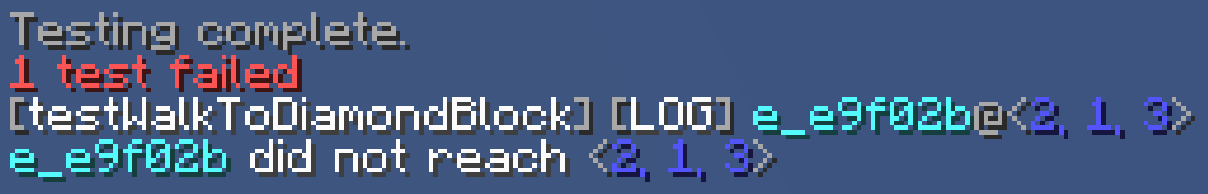
\includegraphics[width=5.89071in,height=0.95353in]{media/media/image6.png}

Figure 4.3.4.2: Report generated in game when an assertion fails.

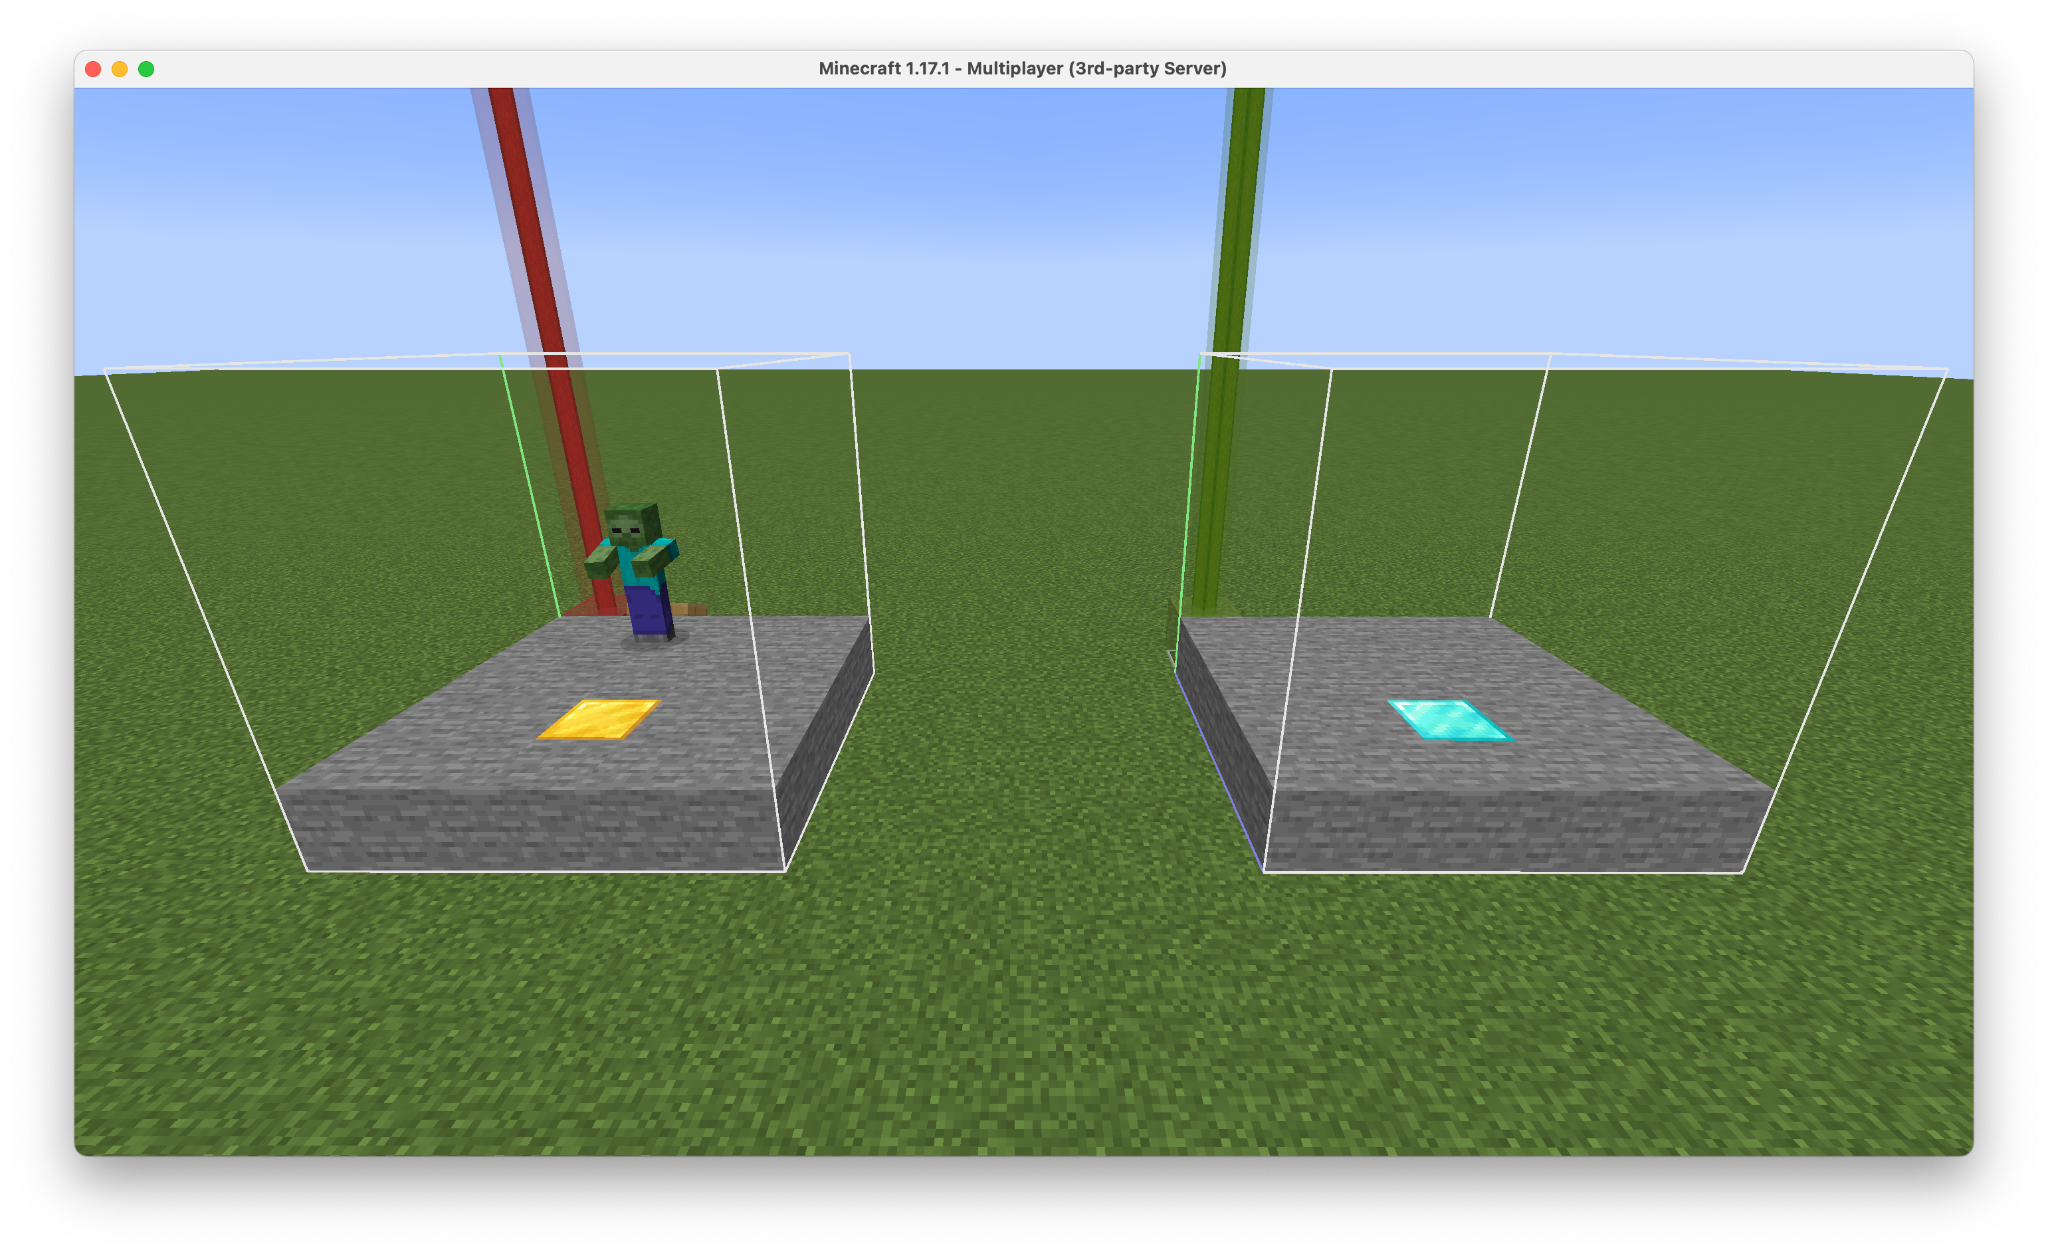
\includegraphics[width=5.89249in,height=3.31771in]{media/media/image3.png}

Figure 4.3.4.3: Red and green beacons indicating success and failure of
a test.

\section{Discussion}

We set out to create an end-to-end testing framework for Minestom
capable of becoming the de-facto standard. Towards this goal, we
addressed many of the challenges associated with end-to-end testing
frameworks, and leveraged the narrow scope of exclusively testing
Minestom applications to create a unique and novel system. To be able to
claim that Canary lives up to the stated goals, we must be able to
assess it in its current state. Beyond that, we must also acknowledge
the places where Canary currently falls short and how Canary might be
expanded in the future to address other goals.

\subsection{Validation}

A library is only as valuable as the benefit it gives users. So when
developing a software library, it is valuable to gather feedback and
opinions from potential users on their thoughts and feelings. On top of
that, a testing library like Canary should ideally be battle-tested and
hardened against all varieties of edge cases. That being said, the
potential user base for Canary is currently quite small. While Minecraft
is a massively popular game, Minestom is a relatively young and new
library, and it will likely be a while until it is a truly viable
alternative for developers creating custom Minecraft servers. That being
said, there are people using and working with Minestom.

Informal conversations with developers using Minestom have indicated
that most do not employ automated testing of any kind. While we believe
that this is all the more reason for Canary to exist, it means that the
validation of the functionality and usability of Canary is limited to a
relatively small demo written by the same people who created Canary.
Creating this demo let us put ourselves in the shoes of someone using
the library.

\subsubsection{Canary Demo}

Canary was designed and built for the goal of testing and entity and
block behaviors and interactions. In order to demonstrate this, we chose
to implement a highly simplified and barebones version of minecarts.
Minecarts are an entity that travels along rails placed by the player.
They can only move along rails, and have a velocity that can be affected
by gravity, or other external forces. Minecarts are a perfect scenario
to demonstrate Canary because they involve interaction between an entity
and blocks in the world.

Our implementation of minecarts is highly simplistic, lacking most of
the features of vanilla Minecraft. What we have implemented is that
placing a minecart on top of a rail will cause it to travel in a
straight line along the rail until it is no longer over a rail. As can
be seen in Figure 5.1.1.1, we created 3 tests for our minecart
implementation.

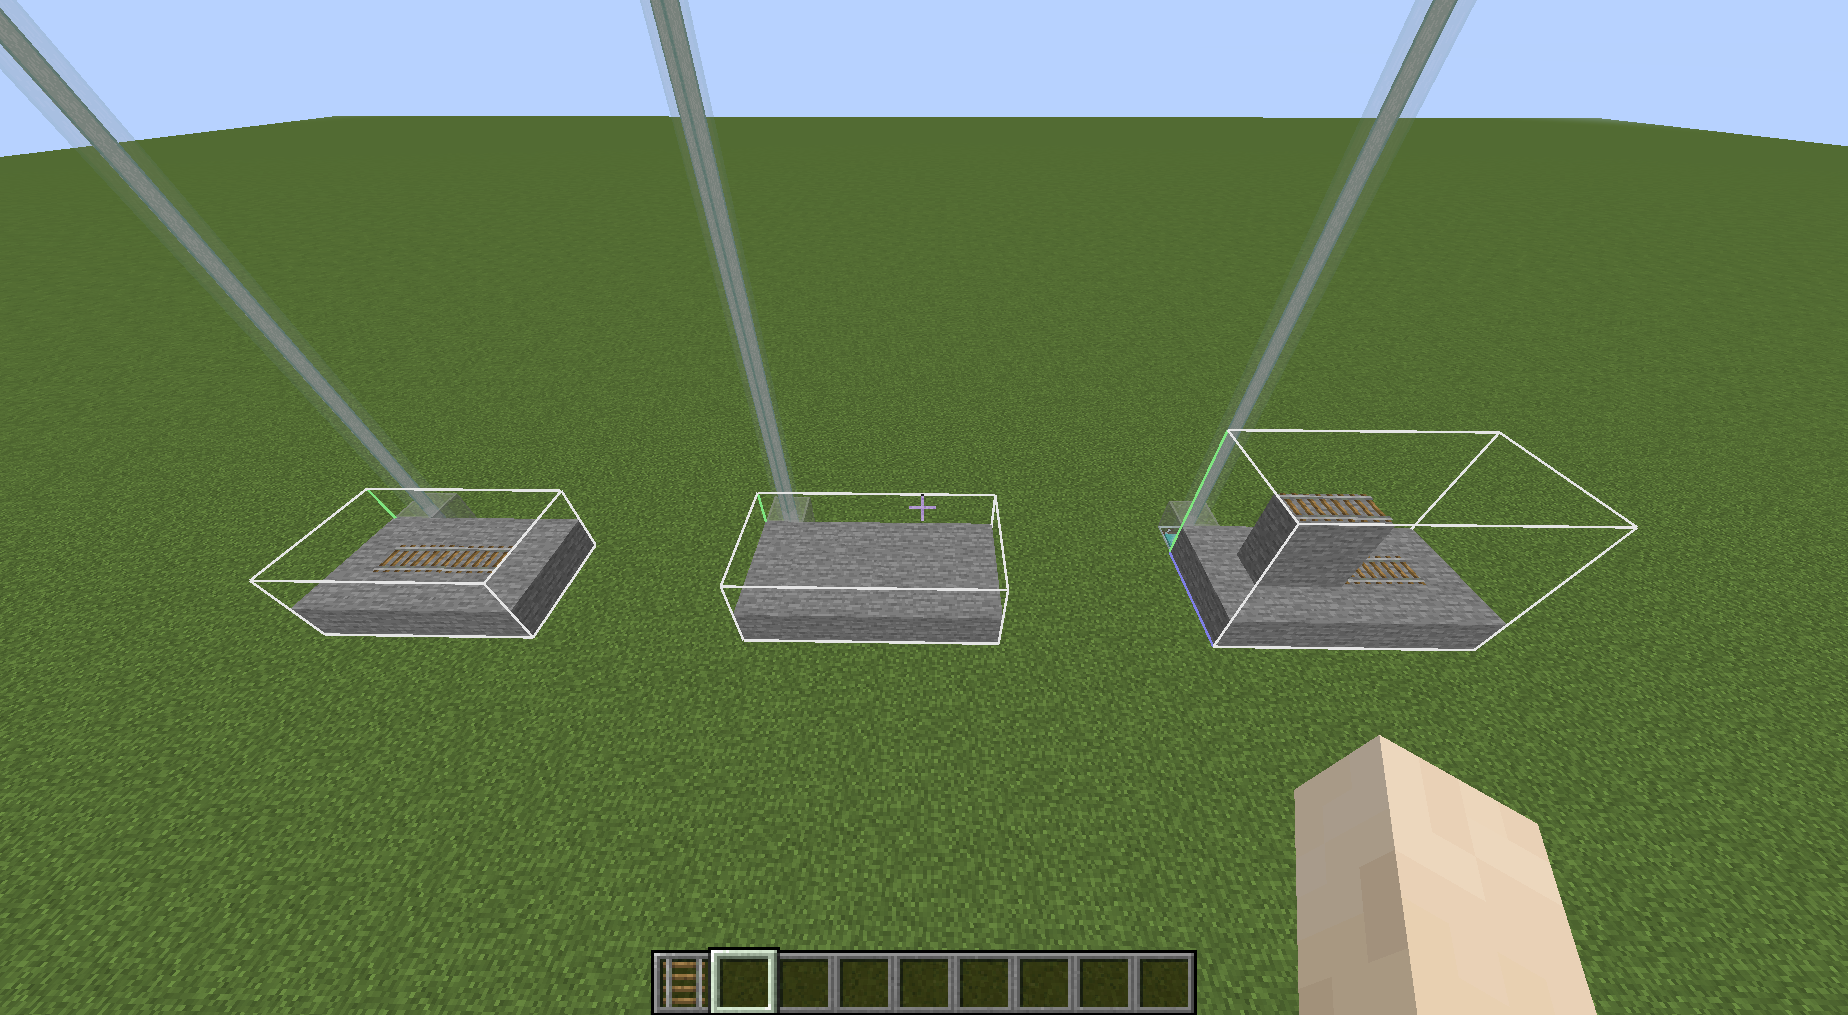
\includegraphics[width=6.14063in,height=3.37538in]{media/media/image15.png}

Figure 5.1.1.1: From left to right, test 1, test 2, and test 3 before
being run

\textbf{Test 1: straight line track}

This test aimed to verify that when a minecart was placed on rails, it
would travel along those rails. The structure for the test consists of 3
rails on top of a layer of stone blocks. The code for this test is shown
in Listing CD.1.

```java

// Listing CD.1

@InWorldTest

public void straightConstantSpeed(TestEnvironment env) \{

// spawns the minecart on top of the first rail (coordinates are
relative to the structure origin)

\begin{quote}
Pos starting\_minecart\_pos = new Pos(1.5, 1, 1.5);
\end{quote}

var minecart = env.spawnEntity(MinecartEntity::new,
starting\_minecart\_pos);

// expect the minecart to be 3 blocks over in the x direction

env.expect(minecart).toBeAt(starting\_minecart\_pos.withX(x
-\textgreater{} x + 3));

\}

```

After running, test 1 passes. Shown in Figure 5.1.1.2 is the test after
passing, with the green beacon to indicate success.

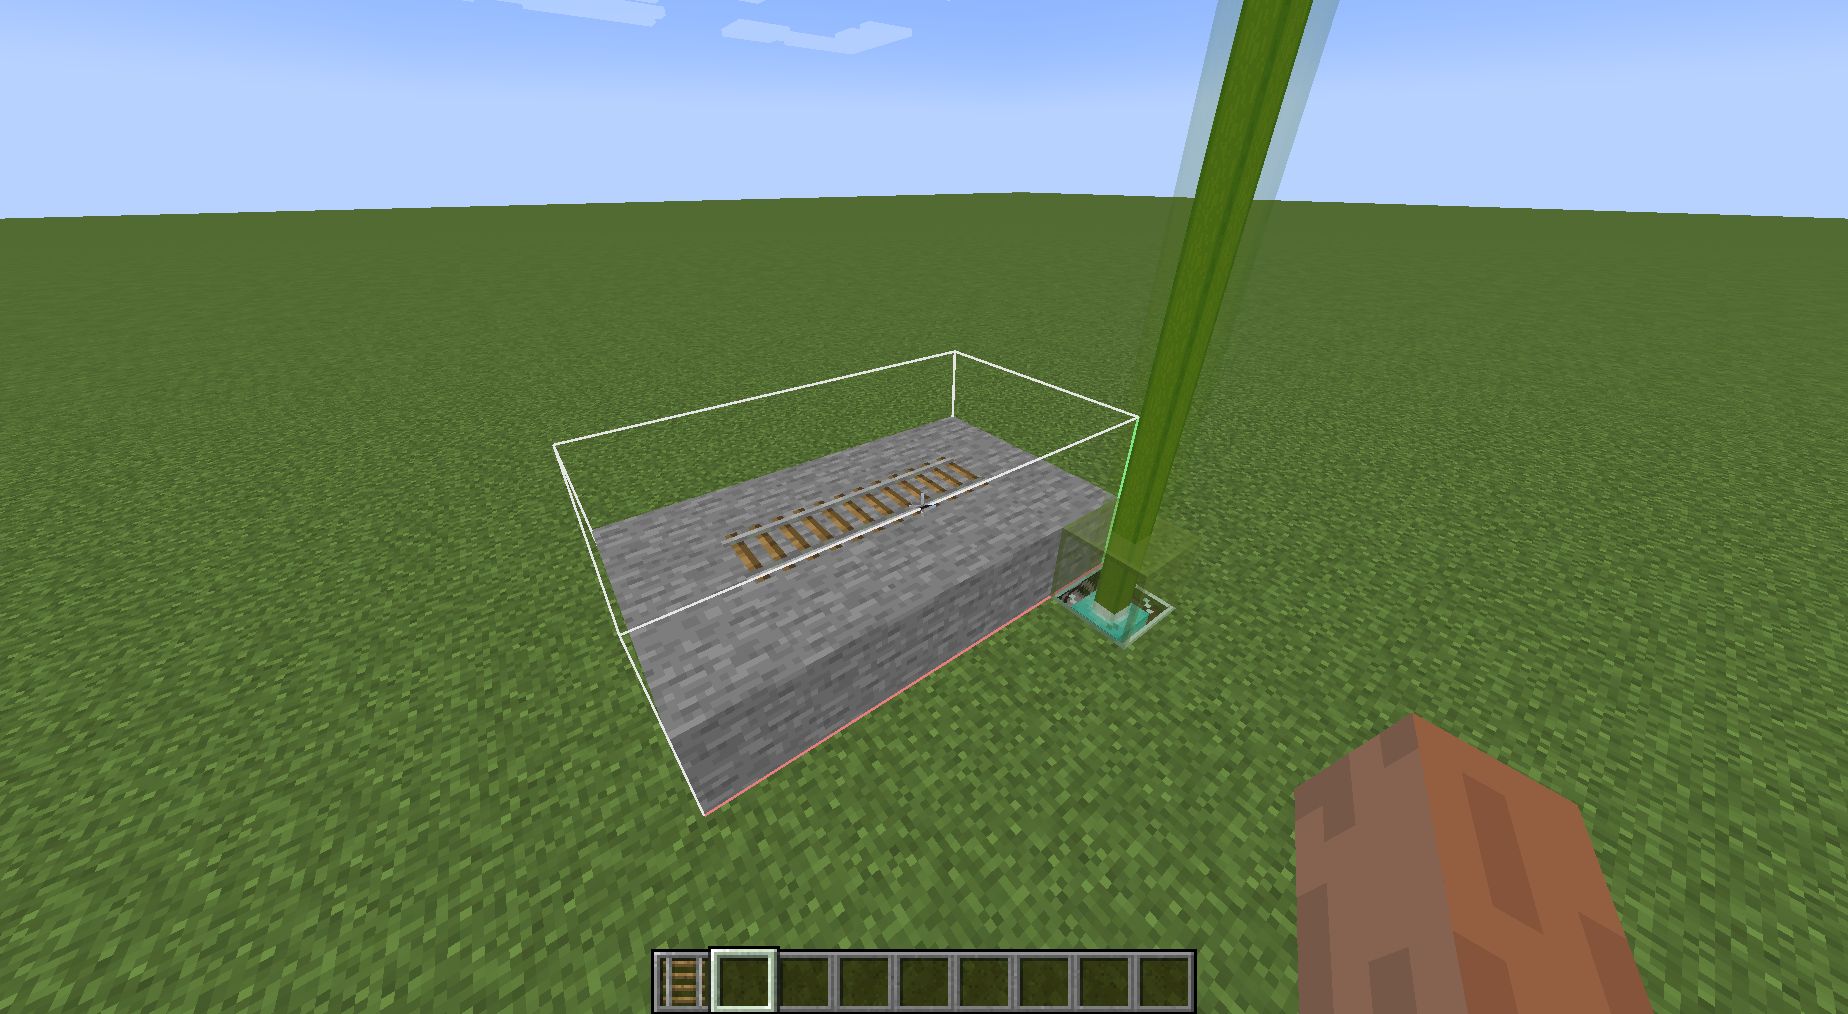
\includegraphics[width=6.17708in,height=3.39355in]{media/media/image12.png}

Figure 5.1.1.2: Test 1 after passing

\textbf{Test 2: No Track}

This test verifies that the minecart only moves forward when it is on
top of rails. The structure and code are nearly identical to test 1,
except the structure associated with it does not have the rails for the
minecart. For the test code, the only change is to the assertion, which
now contains a \code{NOT} (Listing CD.2).

```java

// Listing CD.2

env.expect(minecart).not().toBeAt(starting\_minecart\_pos.withX(x
-\textgreater{} x + 2));

```

This test also passes, although it passes instantly, demonstrating a
current shortcoming of our assertion engine. Because the only assertion
contains a \code{NOT}, the first tick of the test results in a \code{SOFT\_PASS},
meaning the test stops executing. This issue could be addressed by
allowing users to specify a minimum lifetime for the test, giving time
to check for unwanted behavior.

\textbf{Test 3: Gravity}

This tests for a behavior that is currently not implemented correctly:
the ability to fall off one rail and land on another lower down.
Currently, the minecart gets stuck at the top due to incorrect physics
properties.

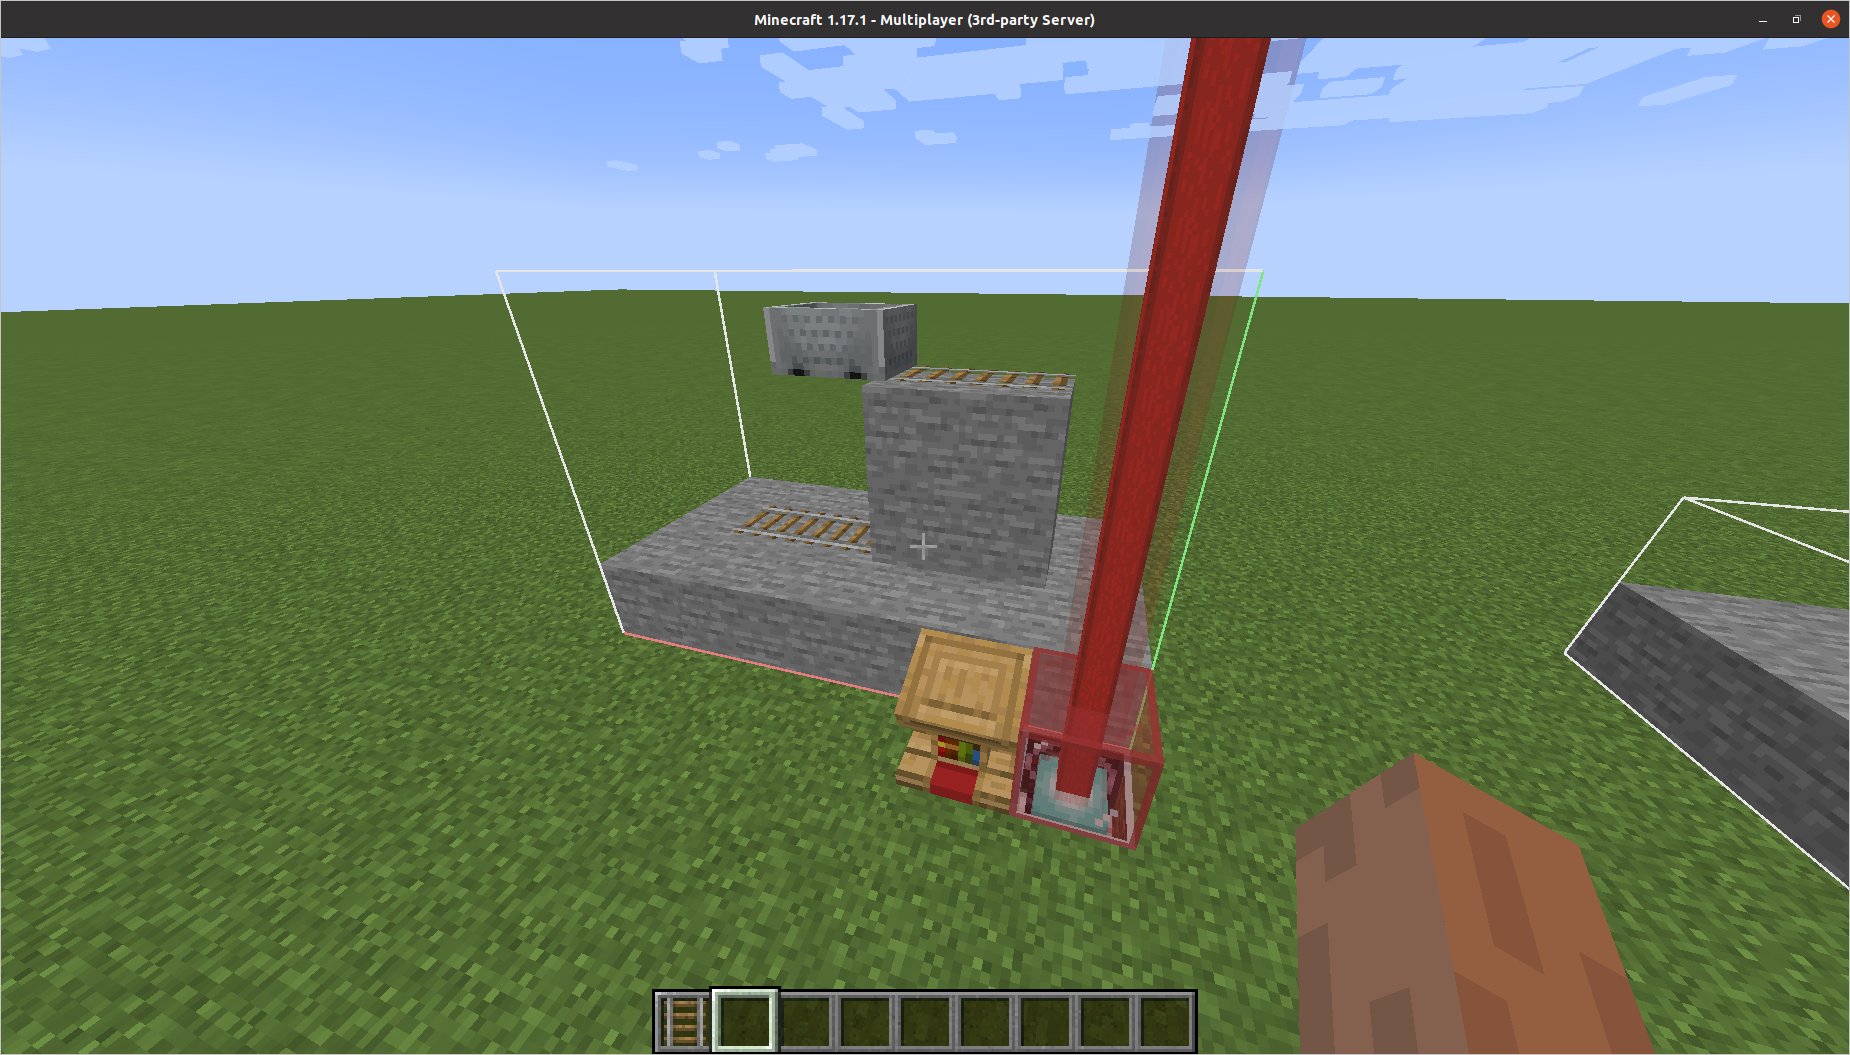
\includegraphics[width=6.5in,height=3.57052in]{media/media/image10.png}

Figure 5.1.1.3: Test 3 after timing out

We see in Figure 5.1.1.3 that when the test fails, the beacon becomes
red, and a book stand is placed. Right clicking on the book stand, as
shown in Figure 5.1.1.4, gives the reason for test failure. In this
case, the test timed out.

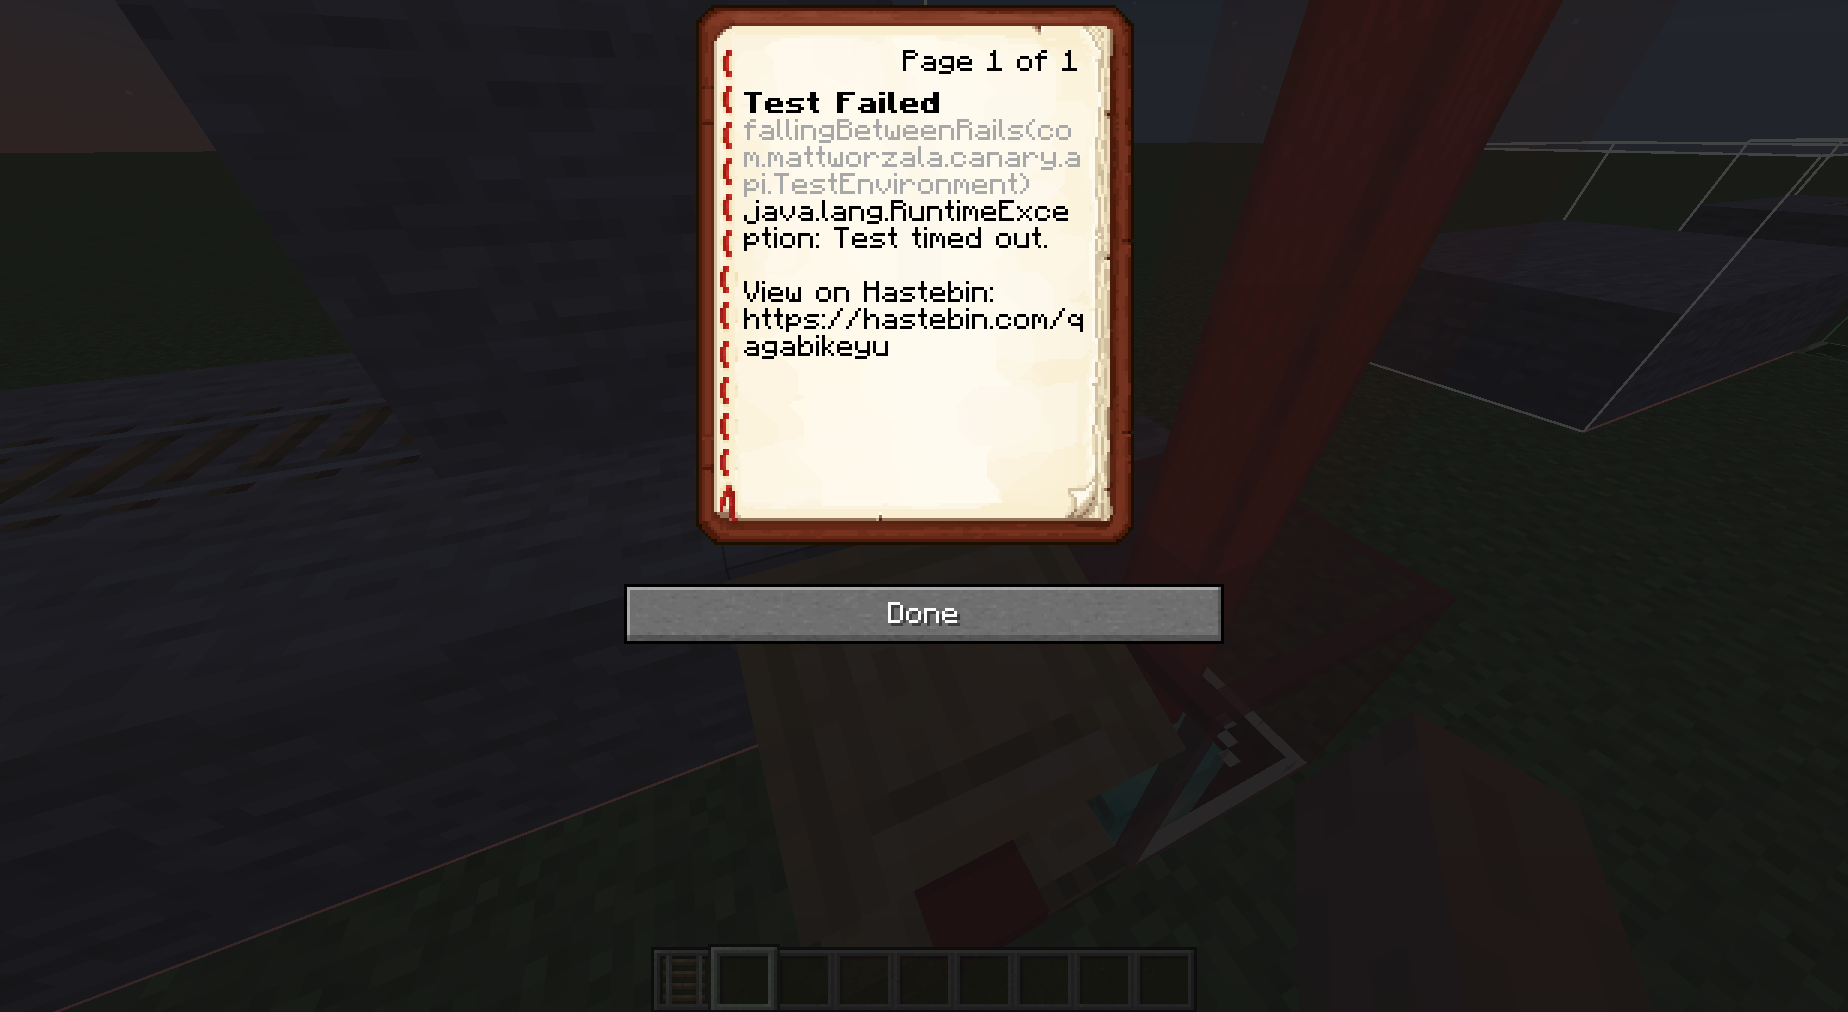
\includegraphics[width=5.8125in,height=3.20414in]{media/media/image14.png}

Figure 5.1.1.4: The error message for test 3

This demo feature implementation and testing shows the basic
functionality of Canary. The process of creating the demo gave us the
opportunity to use Canary like the intended users would. From this
perspective, we found Canary to overall be very usable. Apart from some
bugs and quirks as a result of the somewhat unpolished state of Canary,
all features worked as expected. The test builder, assertion engine, and
test executor do most of the hard work for users, letting them focus on
high level thinking about how to define their tests.

\subsection{Future Work}

Canary implements a usable set of utilities to test many common features
surrounding players, blocks, commands, and entities. However, creating a
fully-featured testing framework for a complex environment like a
Minecraft server is a non-trivial task. There are plenty of features
which would improve the workflow, usability, and usefulness of Canary.

\subsubsection{Unified workflow}

The workflow in Canary involves creating a test structure inside the
game and then switching over to a code editor to write the test code. In
addition, running a test requires restarting the sandbox server or hot
reloading the test code, which is notoriously problematic on the Java
Virtual Machine (JVM). This context switch can cause a reduction in
productivity and can be mitigated. The Mojang GameTest framework uses a
combination of server commands and Behavior Packs (JavaScript) to
execute tests. Using server commands in Minestom can be difficult given
that no server commands are provided by default. As discussed, Canary
introduces a number of utility commands for editing structures in the
test builder; however, they do not extend to replacing test code acting
on the structures. A more fluent solution would allow the user to
``program'' the tests inside the game using the command block feature of
Minecraft. In this case, the tester would be able to edit the tests
without ever leaving the game or worrying about reloading their Java
code.

\subsubsection{Testing Minestom Internally}

Canary has a strong focus on testing applications built on top of
Minestom, and it assumes that Minestom features are properly working. At
the time of writing, however, Minestom does not have strong testing of
internal components. Canary could help fill this gap. Testing internals
are not dissimilar to testing applications built on top, and many
principals would stay accurate. When testing user applications, you may
generally ignore the client because the server acts as an adapter and is
assumed to be working. To test the server, the client must be included.
A system such as the attempt at creating a mock client for Minestom can
test known behavior of the client. Unfortunately, the client is closed
source and written by Mojang, meaning that changes to the client are not
widely published, so features can break at any point. Alternatively,
using a running client to test using the real behavior is both more
accurate, and tests for regression when the client changes internally.

\subsubsection{Behavior-driven Development}

Behavior-driven development (BDD) is a practice similar to TDD where
testing becomes an integral part of the writing process. Where BDD
differs, however, is how tests are written; TDD takes a traditional
approach of self-contained test functions, whereas BDD works in terms of
"scenarios". These scenarios describe a series of events and expected
behavior. A sample can be seen in Listing 5.2.3.1 for a store
application where the scenarios describe what happens to an item when
returned to a store. BDD provides two key benefits: tests which provide
concrete usage examples, and collaboration with non-developers to create
a shared understanding of functionality.

```

// Listing 5.2.3.1

// Adapted from
https://en.wikipedia.org/wiki/Behavior-driven\_development

Title: Returns go to inventory.

As a store owner,

I want to add items back to inventory when they are returned,

so that I can track inventory.

Scenario 1: Items returned for refund should be added to inventory.

Given that a customer previously bought a black sweater from me

And I have three black sweaters in inventory,

When they return the black sweater for a refund,

Then I should have four black sweaters in inventory.

```

In Canary, a user could create a test structure and then write a
scenario for it in the game using a library of statements which have
been defined by developers and Canary itself. This would solve the
context switching issue discussed previously and allow the user to go
from inception to execution all without leaving the game. Furthermore,
since scenarios are designed to be abstract statements of expected
functionality, non-developers could contribute. This could lead to a
workflow where a Canary sandbox is always running, and multiple people
(developers or not) would join to test out functionality and create test
cases while doing so, all working towards a shared understanding of the
intended functionality.

\section{Conclusion}

Canary is a framework with surgical precision in scope. Because it is
created specifically for Minestom, it can integrate extremely closely,
providing users a seamless and easy to use experience. Taking
inspiration from other projects with similar goals, we have created an
end-to-end testing framework capable of becoming the standard for high
level testing in Minestom. Indeed, the methods shown here, particularly
the solution for making assertions on events happening in the future,
could be applied to other projects inside or outside the game
development space. While there is more to improve, Canary has opened up
a discussion about testing in the Minestom ecosystem. It has shown the
community that testing does not have to be difficult or time-consuming,
and it will increase reliability of software considerably.

As of the writing of his paper, Canary has not had a full and complete
release. The project will continue to be developed afterwards,
addressing current issues as well as allowing for new methods of
testing. We have shown it to be a simple framework for testing complex
behavior, and we believe that testing can and will become a standard for
Minestom projects in the future.

\end{onehalfspacing} % Return to single spacing

% \addcontentsline{toc}{section}{References} % Add the 'References' section to the table of contents
\printbibliography
%\bibliographystyle{ieeetr} % Set the bibliography style
%\bibliography{bibliography.bib} % Generate a bibliography from the .bib file with all of the references
%\hypertarget{references}{%
%\section{References}\label{references}}

%To be added in the final version, individual sources are found commented
%in the relevant location.
\begin{onehalfspacing}

\section{Appendix A: Java Classes \& Runtime Modification}

When a Java class is requested by another class, for example by calling
its constructor, the class is loaded into the Java Virtual Machine (JVM)
by a \code{java.lang.ClassLoader}. The language allows multiple class loaders
to exist in a tree, which imposes restrictions on which classes can be
accessed where. Class loaders form a bottom-up tree structure where
class loaders know their parent, but not their children. Using the class
loader setup in Figure AA.1 as an example, class loader A and B both
have a shared parent of the root class loader. All classes must be
loaded into a single class loader, which determines whether they are
able to access other classes. For example, \code{ClassA} is loaded into class
loader A. Classes may \emph{only} access other classes in their own class
loader or in a parent. In this case, \code{ClassA} may access \code{Main} and
`StringUtil`, but \emph{not} \code{ClassB}. In the same respect, \code{Main} may 
not access \code{ClassA} or \code{ClassB}. When a class loader is instructed to 
load a class, it will first attempt to load the class from a parent class
loader, and then try to load it in itself. In Listing AA.1, this means
that if class loader A requests \code{ClassA}, it will return the loaded
version. However, if the root class loader requests \code{ClassA}, a new,
unique, instance will be loaded onto the root class loader. Having
duplicate instances of the same class can cause significant problems
because they are \emph{not} convertible (for example, an instance of
\code{ClassA} from class loader A cannot be assigned to a variable of type
\code{ClassA} from the root class loader). This system is relevant to
Minestom because Minestom uses the Mixin framework.

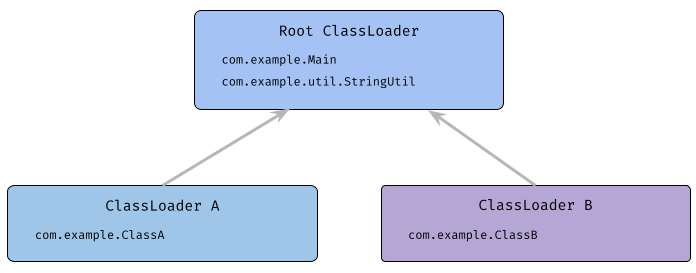
\includegraphics[width=4.71875in,height=1.7856in]{media/media/image1.png}

Figure AA.1: Example class loader hierarchy

Mixin is a framework developed by the SpongePowered team for runtime
modification of Java classes. It hooks into the class loading process to
modify the bytecode of the loading class. This allows a user to modify
an existing class of a library without having to compile a new version
or fork the project. Listing AA.2 shows an example Mixin which will add
a system print to the first line of \code{CanaryTestEngine\#discover} at
runtime. Listing AA.3 shows the definition of
\code{CanaryTestEngine\#discover} at compile time and then at runtime after
the Mixin has been applied. Minestom includes the Mixin framework so
that extensions (Minestom's plug-in system) are able to modify Minestom
classes without requiring a fork of the project.

```java

// Listing AA.2

@Mixin(CanaryTestEngine.class)

public class CanaryTestEngineMixin \{

@Inject(method = "discover", at = @At("HEAD"))

public void discover(EngineDiscoveryRequest discoveryRequest, UniqueId
uniqueId,
CallbackInfoReturnable\textless CanaryEngineDescriptor\textgreater{}
cir) \{

System.out.println("Printed during discovery");

\}

\}

```

```java

// Listing AA.3

@Override

public CanaryEngineDescriptor discover(EngineDiscoveryRequest
discoveryRequest, UniqueId uniqueId) \{

return CanaryDiscoverer.discover(discoveryRequest, uniqueId);

\}

@Override

public CanaryEngineDescriptor discover(EngineDiscoveryRequest
discoveryRequest, UniqueId uniqueId) \{

System.out.println("Printed during discovery");

return CanaryDiscoverer.discover(discoveryRequest, uniqueId);

\}

```

The presence of this system adds a significant complexity to Canary.
Mixin requires that all classes are loaded into a Mixin-enabled class
loader so that it can intercept and modify the classes as they are
loaded. To enable this, Minestom provides a bootstrap class to set up
the Mixin environment and then invoke the developers' main class.
Listing AA.4 shows an example initialization for a Minestom project.
Unfortunately, this system requires that the developer is in charge of
where classes are loaded. Inside a JUnit test engine, this is not the
case. JUnit instantiates the test engine class and manages loading the
discovered test classes into its own class loader. This means that
Mixins will not be applied, and user features using them will likely not
work. To get around this problem, Canary keeps two isolated class
loaders: the JUnit class loader where the test engine is loaded and
working, and the Minestom server class loader where the server and tests
are running. Since test classes are loaded into the JUnit class loader
but executed in the Minestom class loader, they must be reloaded before
execution. This system adds significant complexity and safety
requirements to Canary (see Appendix B); however, it comes with an
advantage past enabling Mixin support. Because the test engine is
independent from the server, it is possible to start multiple
independent Minestom servers which could provide complete isolation
between running tests.

```java

// Listing AA.4

public class BoostrapMain \{

public static void main(String{[}{]} args) \{

// com.example.Main.main(String{[}{]}) will be invoked after being
loaded into the Mixin class loader.

Bootstrap.bootstrap("com.example.Main", args);

\}

\}

```

This project and report were written for Minestom targeting Minecraft
version 1.17. The game is now on 1.18, and during the 1.18 update,
Minestom removed Mixin support. This means that the system will no
longer be required for Minestom versions going forwards unless Canary
itself needs to use Mixins to modify Minestom for any reason.

\section{Appendix B: Tooling}

Canary has some complex systems to manage class loaders and assertions,
but to aid in development and usage, we created some external supporting
tooling. A Gradle plugin and a Java compiler plugin were both created to
help simplify usage and reduce errors. The Gradle plugin is mainly for
external users, whereas the compiler plugin is intended for internal use
only.

The Canary Gradle plugin is a simple plugin to facilitate development
when using Canary in an external project. The obvious task of the plugin
is to set up Canary as a test dependency. Canary should never be added
to the main class path, so it is only set up on the test class path.
Additionally, in the future the API will likely be split away from the
JUnit test engine implementation, creating a more complex dependency
setup. Next, the plugin creates a task to start the sandbox server. The
sandbox server may be started manually by invoking it's main class
(\code{com.mattworzala.canary.internal.launch.SandboxLauncher}); however, there
are some required command line arguments which would have to be added
manually. These options are configurable through the Gradle plugin. An
example usage can be seen in Listing AB.1. The plugin is added via its
ID (\code{com.mattworzala.canary}) and then may be configured through the
canary block. In this sample, only the Canary version is being
configured.

```kotlin

// Listing AB.1

// build.gradle.kts

plugins \{

id("com.mattworzala.canary")

\}

tasks \{

canary \{

version = "-SNAPSHOT"

\}

\}

```

While the Gradle plugin facilitates external usage, there is some room
for internal tooling as well. As described in Appendix A, Canary
requires strict isolation between the JUnit Classloader and the Minestom
Classloader. As such, a reference to a JUnit class, such as
CanaryTestEngine (the JUnit engine implementation) is invalid from a
Minestom server class, such as \code{HeadlessServer}. To prevent accidental
references, we created a Java compiler plugin to enforce this isolation.
A Java compiler plugin is similar to an annotation processor; however,
it is given direct access to the Abstract Syntax Tree (AST) and may
manipulate it with much more freedom. The downside, however, is that the
\code{javac} Application Programming Interface (API) does not have the same
backwards compatibility guarantees as the annotation processor API. In
this case, a compiler plugin is required because annotation processors
do not have access to import statements. The Canary compiler plugin (or
safety checks) works by looking at import statements and the @Env
annotation. The annotation is used on class definitions and tells the
safety checker what environment (class loader) the class may be used in.
The valid options are \code{GLOBAL} for classes available in both class loaders
and \code{PLATFORM} / \code{MINESTOM} for JUnit/Minestom respectively. With this
information, errors can be generated from invalid import statements.
Figure AB.2 shows an error generated by the safety checker when
importing \code{CanaryTestEngine} from \code{HeadlessServer}.

```

// Figure AB.2

HeadlessServer.java:6: error: Cannot import com...CanaryTestEngine
(PLATFORM) from MINESTOM

import com.mattworzala.canary.internal.junit.CanaryTestEngine;

\^{}

```

\end{onehalfspacing} % Return to single spacing
%\section*{Abstract} % Start the section 'Abstract'. Include the asterisks to keep section unnumbered and off of the table of contents

%\noindent Type abstract here. % Use '\noindent' to remove indentation from the first paragraph of each section
%\par Second paragraph of abstract % Use '\par' to start a new paragraph

%\newpage % Start new page
%\section*{Acknowledgements} % Start the section 'Acknowledgements'. Include the asterisks to keep section unnumbered and off of the table of contents

%\noindent Begin list of acknowledgements
%\begin{enumerate} % Start a numbered list
    %\item First Acknowledgement % Name of first acknowledgement
    %\item Second Acknowledgement % Add new item with '\item'
%\end{enumerate}

%% OR %

%\begin{itemize} % Start a bulletted list
    %\item First Acknowledgement % Name of first acknowledgement
    %\item Second Acknowledgement % Add new item with '\item'
%\end{itemize}

%\newpage % Start new page 
%\tableofcontents % Table of contents
%\listoftables % List of tables
%\listoffigures % List of figures

%\newpage % Start new page
%\begin{doublespacing} % Adjust spacing
%\pagenumbering{arabic} % Set page numbering to Arabic numbers
%\setcounter{page}{1} % Set page number to 1

%\section{Introduction} % Start the section 'Introduction'. Do not include the asterisks to add section number and include in table of contents

%Minecraft is a popular video game developed by Mojang studio and officially released in 2011. The basic premise is that the world is made up of many cube shaped blocks, and the player has the ability to break and place these blocks. Since its first release, Minecraft has grown into something much larger than this basic premise. One part of this growth is through custom multiplayer servers that allow for entirely new ways to play the game. Traditionally these custom servers have been accomplished by in some way modifying the default multiplayer server. This has been a very fruitful approach, and there are a massive amount of servers that take this approach. 

%Minestom is an open source library that re-implements the basic functionalities of a Minecraft server. The goal is to provide a strong foundation for people to build custom Minecraft servers on top of. Minestom is more performant, and far easy to extend than the default server, because it was built from the ground up with those goals. People who want to create a custom multiplayer gamemode or any other sort of custom behavior, can choose to build it on top of Minestom instead of using other tools that work by modifying the default multiplayer server. Since Minestom is a library that is aimed at people who want to implement custom functionality, providing a robust software development framework is important. Part of this framework could include test driven development. 

%Test driven development is a software development methodology where the software requirements are first encoded in test cases, before they are implemented. This means that you can continually test your software using the test cases, and have some reassurance that it is working correctly. This is commonly done using unit tests, which are tests of specific parts of the code like a class or function. This specificity is great for making sure that particular parts of a larger system are working properly. They are something that are simple to integrate into a java codebase using libraries such as JUnit. For when you want to test the behavior or functionality of an entire system, integration tests, or end to end testing are the solution. In other contexts this may take the form of automatically clicking through buttons on a form to ensure that it reaches the correct end state, or doing a predetermined set of inputs into a video game, and verifying that you end up where you expect to. 

%Minecraft presents a particularly interesting situation with regard to end to end testing, in that everything is modular and intended to behave the same in many different situations. You can manually test a feature by building some test structure, and then taking steps like spawning entities, or interacting with blocks, to test the feature. You would look for the expected behavior, and then be able to determine if the feature works as expected. This is a workflow that can be automated. You can build your test structure and then save it. Then you can use the test structure along with programmatic equivalents of the additional steps like spawning entities, or interacting with blocks. Then you can have assertions about the behavior of the situation under test. 

%%\newpage % Start new page
%\section{Background}

%Test driven development has become a popular technique in recent years, and as such this project is not the first to attempt to bring testing into the Minecraft world. Mojang itself has created an internal tool (named GameTest) for testing their game, and it serves as a great inspiration for this project. According to Henrik Knilberg (2020), a member of the gameplay team at Mojang, “”. Ultimately, while Mojang’s work serves as a good inspiration for creating tests based inside the game, it has some significant flaws for widespread use. It is not made for Minestom, and therefore makes a number of assumptions about Mojang features being implemented. Furthermore, the framework is closed source, so modifications are challenging and ineffective in a different environment, and cannot be posted publicly. In the category of modifications to the Mojang server, there have been two major attempts at testing: MockBukkit and McTester. Both take a programmatic approach to testing, and target different use cases. MockBukkit provides the user with an API for creating mocked resources such as players, worlds, and Bukkit plugins. This approach does allow for a variety of testing methods, however, since the tests are created programmatically, the setup can be expensive even for simple tests. McTester works by running a headless client and allowing the test to submit commands to the client, which can be asserted on server side. For example, a test could include a client right clicking a Command Block and asserting that the GUI was only opened if the player had appropriate permission. This method of end-to-end testing is effective for testing a server implementation (such as testing Minestom internally), however, it introduces unnecessary overhead for testing applications built on top of Minestom because the internals are expected to be tested and working independently. Finally, Minestom has seen its own attempt to create a testing framework internally. The test framework involved a mocked client connection to the server, from which a test could submit packets and make assertions on the received packets. Similar to McTester, this can be effective for testing internal features, however, it becomes cumbersome to work on a packet level when testing in userland.

%Custom Minecraft servers have evolved throughout the years, starting from simple survival servers with extra enchantments, to game modes which look and feel like a new game completely.  
%%========================%
%%   Inputting a table    %
%%========================%

%%\begin{table}[!tb] % Use '!' to override the LaTeX table placement, 't' to place the table at the top of the page, and 'b' to place the table at the bottom of the page if the top does not work
    %%\begin{center}
        %%\begin{tabular}{ |c|c|c| } 
            %%\hline
            %%cell1 & cell2 & cell3 \\ 
            %%cell4 & cell5 & cell6 \\ 
            %%cell7 & cell8 & cell9 \\ 
            %%\hline
        %%\end{tabular}
        %%\caption{Caption of table} % Automatically adds a table number which updates as more tables are added to the paper
        %%\label{table:label_of_table} % Used in the paper to reference the table and automatically includes the table number in the in-text reference.
    %%\end{center}
%%\end{table}

%%\par To reference a table, you would simply say Table \ref{table:label_of_table}. By using the table label, the reference updates automatically as the paper is edited and more tables are added.

%% For more information, go to https://www.overleaf.com/learn/latex/tables

%\section{Requirements}

%\subsection{Objectives and Constraints}


%As previously discussed, this project aims to fill a perceived void in the minestom ecosystem for end to end testing solutions. We hope to create a library to be the de facto standard for end to end testing in the Minestom ecosystem. In order to meet this goal, we need to consider two main factors, ease of use and coverage of all major use cases. Ease of use means that developers using Canary shouldn’t feel like they have to fight with the library in order to accomplish what they want. The library should be internally consistent and predictable, while handling the needs of developers. To cover all major use cases, Canary should be applicable to the scenarios where developers would want end to end testing.

%To figure out what standard usage might look like, we can look towards the greater Minecraft server modding community to see what sort of features or functionality people have implemented within a Minecraft server.

%Although the functionality and features that people add to Minecraft servers are broad and diverse, we can break them down into a few general categories based on what they require from an end to end testing library. The main factor in determining what a feature requires to be able to be tested, is the types of effects on the world it can have. We will look at three broad categories of functionality that can be added to a minecraft server.


%\noindent \textbf{Custom entity or block behavior}

%This category refers to most world behavior that is not linked to the player. This includes entity AI, entity properties, block properties, and how blocks interact with other blocks, and more. Generally these features only affect a small area around the block or entity, and happen based on the state of the world, and not players in the world. 

%Manually testing these types of features would generally involve building some sort of setup that will cause the desired behavior to occur, and then watching for the behavior to happen as expected. If testing, for example, you want to test that minecarts roll down hills correctly. You would first build a track down a hill, and then place a minecart on that track. Then you would watch for the minecart to end up at the bottom of the track. 

%Canary should allow you to define the setup for a test, as well as the expected outcome, and then execute the test on its own.  The required functionality for this is:
%Be able to define the starting state of a test, including the blocks, block properties, and entities.
%Be able to check if expected outcomes happened. 

%Determining if the expected outcome happened, in general, is a challenging problem. There is a wide variety of things that someone might look for to determine if a test ran correctly. Examples include, looking for an entity to get to a location, looking for a block to be in a certain state, making sure some condition did not happen, or checking for things to happen in a certain order. There is a further discussion of  assertions in the needs section.

%This category of feature is likely the one that benefits the most from end to end testing. Because most of the behaviors only cause changes in a small area, tests can be run simultaneously without having to reset the entire world between tests. On top of the functionality requirements, the process of making, running, and debugging these tests should be simple and straightforward to align with the overall goal of ease of use.

%\noindent \textbf{Custom server commands}

%Server commands are a way to use player messages like a command line or terminal. Custom commands are a common way to implement features like switching between worlds, primitive UI for server interaction, or a way for players to modify various aspects of the world. Server commands, unlike entity and block behavior, frequently affect things far beyond the player, including internal server state. To test server commands we should be able to 
%Simulate a player from a known starting state in a known context executing a command
%Check for the expected behavior of the command

%Server commands present a particular challenge in that their behavior is not bound in any way. A server command can do anything from changing a block near the player, to teleporting the player, to affecting other players, worlds, or the entire server. This broad scope makes it challenging to be able to effectively test all varieties of server commands, because creating a known starting state could potentially require restarting the entire server between every test, which would seriously impact the ability to quickly run tests.

%\noindent \textbf{Customizing player interaction}

%As discussed, changing what happens when a player interacts with the world is quite a common thing for Minecraft server mods to do. The types of changes that might be caused by these custom player behaviors frequently cover the full range of possible server behavior. Anything from combat, to inventories, to manipulating custom guis.  Similar to server command, testing player interactions requires
%Simulate a player from a known starting state in a known context interacting with the world in some particular way
%Check for the expected behavior of the interaction

%Player interaction often causes changes that can be challenging to test. A player clicking on an item in their inventory might teleport them to a different world, or a player clicking on a block with a certain item could cause that player to be sent a chat message. 

%\subsection{Final Requirements}

%Over all, there are many challenges to creating a test system that covers all expected use cases. In particular, being able to test every possible server behavior in a consistent and reliable manner would force the overall library to be much less useful. For this reason, we chose to focus mainly on testing custom entity and block behavior features which can be tested in a finite and confined area. These features can require elaborate setups to fully test, and stand to benefit the most from automated end to end testing. That being said, we have not entirely ignored other feature types, and they could be the focus of future work, or other projects.

%From this, we can create a list of the high level requirements of Canary. We have split the requirements into two categories, based on our original goals of ease of use, and full feature coverage.

%\noindent Ease of Use 
%\begin{itemize}
  %\item Canary must be easy for developers to use, including creating tests, running tests, and debugging why a test might have failed.
  %\item When possible, Canary should allow developers to create tests in a way similar to how they would when manually testing
  %\item The code API used when writing code for tests should be understandable and abstract away common operations
  %\item When a test case fails, Canary should provide error messages that help debug the problem
  %\item Tests should be fast to run on a local machine
  %\item Tests should be able to run in CI/CD servers in the same way other types of test might
  %\item Any data for tests that is not code should work nicely with version control
%\end{itemize}
%\noindent Feature Coverage

%\begin{itemize}
  %\item Canary must be applicable to all major use cases, in particular custom block and entity behavior should be able to be tested by Canary.
  %\item Defining the expected outcome of a test should be able to express complex scenarios
  %\item The things that can be asserted about should by default cover most common usage, and allow for easy developer extension for rare or custom properties
%\end{itemize}
%%========================%
%%   Inputting an image   %
%%========================%

%\par To add an image to the document, you first have to upload it to the file. To do so, click the "Upload" button on the top left of the screen (just below the "Menu" button, pictured in the figure below) and upload the image from your computer. 

%\begin{figure}[h] % Use 'h' to tell overleaf to place the image approximately 'here', meaning that you want it to be somewhere near where you are putting it in the text but will allow LaTeX to move it so that the overall format is best
    %\centering
    %
\includegraphics[width=0.5\textwidth]{Images/logo.png} % Set the image width relative to the with of the text on the page and input the name of the image that is being placed.
    %\caption{Figure Caption} % Automatically adds a figure number which updates as more figures are added to the paper
    %\label{fig:label_of_figure} % Used in the paper to reference the figure and automatically includes the figure number in the in-text reference.
%\end{figure}

%\par To reference a figure, you would simply say Figure \ref{fig:label_of_figure}. By using the figure label, the reference updates automatically as the paper is edited and more figures are added.

 %For more information, go to $https://www.overleaf.com/learn/latex/Inserting_Images$

%\section{Needs}

%With the high level requirements determined, we now have to translate them into specific requirements to be implemented in software. To do this, we first need to decide on our overall approach to end to end testing. For this, we looked at prior work in end to end testing, as well as how developers approach manual testing. Our main inspiration was the work that Majang themselves had done. The key concept from this work is the combination of code with other data to create the “structure” associated with the test, and to use code to define any additional starting setup, as well as to create the assertions for the test. 
%% TODO: some pictures of these test structures, and code for a test

%This approach allows for the creation of the test structures to be done in Minecraft, the same way that someone would when manually testing. Along with this, it should reduce the amount of code needed for each test, further improving ease of use. The actual functionality of Canary can be split up into 3 broad categories that are responsible for all of the requirements.

%\subsection{Test Builder}
%As discussed, Canary tests have a test structure associated with them. This structure is not defined by code. Instead, it is other data that is loaded into the world when a test is being run. To make Canary easy to use for developers, we need to allow them to create these structures in the same way that they would when manually testing, by building them in Minecraft. The test builder is the subsystem of Canary responsible for letting users create and manipulate these structures. The test builder is a feature accessible on servers running Canary, and allows users to build structures in game, that will then be saved in a form that can be ingested when running tests.  

%The requirements of the test builder in general are to allow for creating all the necessary starting conditions for tests. The test builder should also be easy to use, and allow for all of the types of operations that would frequently be needed when making end to end tests. Such as making tests that have similar test structures. The created structures should also allow users to edit the properties of the blocks, either to change how they behave, or to mark them so their position can be referenced from the actual code associated with the test (mark a block with a name that can be used to easily get the position of the block).

%Once a user has built a test structure in game, they should be saved in a format that can be read back in when running tests. Additionally, this format should have some amount of compatibility with git. Structure files should be text based so that minor changes to the structure will not cause git to see the whole fill as changed, and instead see a few lines out of the entire structure as changed. 
%\subsection{Assertions}

%Assertions, along with the other API’s involved in the code for each test, are perhaps the most integral part of Canary. The test builder is how a user defines the starting block configuration for their test, and assertions are how a user defines the expected behavior of the test. This system bears the brunt of the complexity in Canary with respect to being fully featured and easy to use. 

%As discussed previously, most other end to end testing systems require the programmer to handle the fact that their tests are most likely not fully deterministic due to factors such as frame rate. Minestom falls into this category, it’s very possible to write code that produces slightly different output depending on things like exact frame timing. For Canary to be useful, we need to provide developers a way of specifying the expected behavior of their tests. To be reliable, this needs to be done without using methods such as directly comparing runs, or letting users prescribe an exact amount of time that something will take.

%The solution proposed in this report is to allow for developers to create small programs that define the expected state of the world during the test. The types of things that can be expected would be that an entity makes it to a certain location, or that there is not a block at a certain position. Additionally, these sorts of assertions can be combined in various ways, such as with a logical and, or by saying that one should happen before the other. This solution creates many challenges, but ultimately it is the only approach that offers the needed capabilities while still fulfilling the other goals of the project.  
%\subsection{Test Executor}
%The test executor is the core of Canary. Similar to other systems, test execution comes with its own set of challenges. These mainly have to do with the need for tests to not affect each other, while wanting the user experience of Canary to be as good as possible. So the main requirement is that a test cannot inadvertently change the results of another test. This would be a risk if tests were run together in the same world such that an entity might react to other blocks outside of the test that it is a part of.

%While we want tests to be isolated, we also want it to be easy for a user to see groups of related tests at the same time. This is a valuable feature both for development when you would want to make sure that all of the tests for a feature are working as expected, but also for when you want to see if groups of related tests are failing in the case of a bug. The way that we have decided to accomplish this is by grouping tests from the same test class together in rows in the world.

%The final feature of the test executor is that it should be able to run the tests both locally, as well as on a CI/CD server. In both cases, there should be output that is helpful in the case of test failure. 


%\section{Implementation}

%As established, writing assertions about events which have not happened, nor will happen in a deterministic manner creates a significant challenge. The solution proposed in this report is split into two distinct segments, roughly modeled after a typical interpreted programming language: assertions themselves (syntax), and the backing assertion nodes (AST). A typical assertion in Canary might look like the following:
%\begin{lstlisting}[language=Java]
%// Listing AE.1
%expect(myZombie).toBeAt(3, 1, 3).and().toHaveHealth(20.0);
%\end{lstlisting}

%%```java
%%// Listing AE.1
%%expect(myZombie).toBeAt(3, 1, 3).and().toHaveHealth(20.0);
%%```
%%The syntax is legible like plain English, eg "I expect that my zombie will be at \bra{3,1,3> and have 20 health". In this report, an assertion may be re\phierenced using the \phiollowing abstract representation:
  %%\verb|EXPECT(myZombie) pos=<3,1,3> AND health=20.0| 
  %%`EXPECT(myZombie) pos=<3,1,3> AND health=20.0`, or simply `pos=<3,1,3> AND health=20.0` for the general case. When the test containing Listing AE.1 is executed, the calls generate a list of steps to the assertion. This step is analogous to tokenizing an input source in a programming language. In this case, the list would be the following:
%%```
%%SUBJECT = myZombie
%%STEPS = [
  %%subject.pos == <3, 1, 3>,
  %%AND,
  %%subject.health == 20.0,
%%]
%%```
%From this list, the engine generates a tree of nodes, each of which has the ability to report whether it passed or failed depending on the condition (eg `subject.pos == <3,1,3>`) or the children. For example, the `AND` node has the following simple logic:  \\
    %1. If any child is a \verb|FAIL|, return `FAIL`
    %2. Return `PASS`
    %%1. If any child is a `FAIL`, return `FAIL`
    %%2. Return `PASS`
%This system is analogous to an Abstract Syntax Tree (AST) in an interpreter, and allows the test executor to simply check the root node to determine the result of the assertion.

%\subsection{Soft Pass}
%%The assertion engine as described above is effective, however, it is not perfect. A common assertion tool is the `NOT` statement. This allows the user to invert the statement directly following. For example, `NOT health=20.0` says that it will fail if the subject's health is equal to 20. Unfortunately, the opposite side is not as simple. Assertions are executed every server tick until they return a `PASS` (more on this later). If, for example, the subject has a starting health of 10, then on the first frame this assertion will return `PASS` and never be tested again. The solution to this problem is to introduce a third state to the equation: `SOFT_PASS`. A soft pass indicates that the condition is currently passing, however it could fail in the future so it must be tested again. This system allows for statements which cannot produce a final output. Another use case of this system is the `ALWAYS` statement. It says that the following condition _must_ be true for the duration of the test. The `ALWAYS` node can never return a `PASS`, because the condition could still change in the next tick, so instead it returns `SOFT_PASS`.

%\subsection{Assertion Specification}
%TODO: Finish in iA

%\subsection{Player Interaction Testing}
%TODO

%\subsection{Test Executor}
%The Canary test executor is responsible for managing the testing environment and complying with the JUnit test engine specification. When the engine is invoked, it first discovers every potential test case (method annotated with `@InWorldTest`). Each test is loaded into the appropriate Java ClassLoader (TODO: Talk about class loaders. It is relevant because we are targeting mixin Minestom. Could put this in an appendix and talk about the ClassLoader troubles as well as the compiler plugin that ensures nothing bad is happening), and a Minestom "instance" is created. An "instance" in Minestom is analogous to a Minecraft world, and allows the test to be completely isolated from all others. When the tests are executed, each test structure is placed into its respective instance, the assertion engine parses the step lists (Listing AE.2) into assertion trees. Finally, the test instances are ticked until it receives a definitive result. The stop conditions for a running test are as follows:
  %%1. Every assertion has returned a `PASS` value (pass)
  %%2. Every remaining assertion returns a `SOFT_PASS` value (pass)
  %%3. The timeout limit has been reached (fail)

%%A definitive pass may happen in two cases:
  %%1. Every assertion returns a `PASS` value
  %%2. The test times out and every remaining assertion returns a `SOFT_PASS` value.
%%The second condition is due to the behavior of `SOFT_PASS`. An assertion such as `ALWAYS` cannot ever know that it has definitively passed, so it exclusively returns `SOFT_PASS` or `FAIL`. When a test times out, however, it means that there are no more steps so a `SOFT_PASS` is equivalent to a `PASS`. Because Canary tests run over a long period of time and state changes throughout, `FAIL` does not indicate a definitive failure. Instead, it indicates that the test has _not yet passed_ but may in the future. If the time runs out and there are still failing assertions, then the test is a failure.

%\subsection{Sandbox Instance}
%Writing tests inside the environment they are testing provides the user a huge benefit, including real-time feedback. The user can enter the game and watch their tests running in real time, making it extremely simple to determine what is wrong. Canary facilitates this using the "sandbox instance", a Minestom instance containing every loaded test. This world allows the user to visibly see which tests are passing or failing, and fly around to view them.

%\subsection{Sandbox vs. Headless Mode}
%Canary has a strong focus on ease of use and visual feedback through the sandbox mode of the test engine. That, however, is not the only responsibility of a test engine. Test engines must be able to execute remotely in a Continuous Integration/Continuous Development (CI/CD) pipeline. Canary refers to this execution mode as "headless" mode, and it differs from the sandbox mode in a few ways. The running test server is not available to join, and the debug information is not loaded including commands and the sandbox instance. To ensure that all tests remain isolated and predictable, each test is still loaded into its own instance.

%\subsection{Isolation}
%It is critical to create the same exact environment for every execution of a test both locally on multiple distinct machines, or remotely as a part of a CI/CD pipeline. This task is non-trivial in the Minestom environment, since a test may access and use arbitrary server data, or interact with arbitrary blocks around the test environment. The most obvious solution is to use a unique Minestom server for each test which solves the global state and nearly interaction issues simply. Unfortunately, this solution has significant drawbacks in terms of speed and usability. Minestom makes use of some global (`static` in Java) state for running server information, which means that you cannot easily have two Minestom servers running at the same time. It is possible to start a Java Virtual Machine (JVM) subprocess for each test, or to load each test into its own ClassLoader. Both results incur a large initialization overhead and memory increase for each individual test because every class must be reloaded each time. Regarding usability, separating each test into its own JVM or ClassLoader means that it is no longer possible to create the aggregate sandbox instance, destroying the ease of creating tests. Instead, Canary handles isolation by placing each individual test (and associated structure) into its own unique Minestom instance. This allows the sandbox instance to remain by forwarding actions from each sub instance into the sandbox. This solution, however, does not impose strict isolation for global server state. In the end, this compromise was worth the benefit provided by the sandbox instance. One of the benefits of thorough testing is that it forces users to write code which can be used in isolation, so this requirement is helpful in some ways.
%%========================%
%% Inputting an equation  %
%%========================%

%% Use '\begin{equation}' to input a numbered equation. Used when equations will be reference in-text. Unlike tables, this equation will appear exactly where you put it in the text.

%%\begin{equation} 
    %%y=mx+b
    %%\label{eq:equation_label}
%%\end{equation}

%%\par Once the equation is inputted, you can reference it similarly to tables using 'Equation \ref{eq:equation_label}'. Just like tables, the equation number update automatically when the paper is edited and new equations are added. 

%%\par If you want to include an equation that is not numbered, use the form $$\frac{-b\pm \sqrt{b^{2}-4ac}}{2a}$$ and the equation will appear exactly where you put it in the sentence, in it's own line. 

%%\par If you want to include an equation in a sentence without putting it in its own line, use the LaTeX 'math mode' using the form $x_{1}^{2}+x_{2}^{2}=r^{2}$. 

%% For more information and different methods, go to https://www.overleaf.com/learn/latex/mathematical_expressions

%\section{Conclusion}

%\noindent Input your conclusion here. 

%\par Notes: 
%\begin{enumerate}
    %\item The table of contents is set up with hyperlinks, and you can get to any section of the paper by clicking the section in the table of contents. Same for tables and figures. 
    %\item You can input as many sources as you want into the .bib file. They will only appear in the 'References' section if they are cited in text. The 'References' section is organized in the order of which the sources are cited in text. The in text citations are also hyperlinked, and clicking one will bring you to that source in the 'References' section. 
    %\item If you ever don't know how to do something, you can almost always find it on \url{https://www.overleaf.com/learn} or just by Googling. 
    %\item The paper can be split into sections, subsections, and subsubsections, and subsubsubsections. These can be inputted in any part of the main body of the text, from the abstract to the conclusion. Adding an asterisks in the command line will prevent the section from getting a section number and appearing in the table of contents.
    %\item Appendices are referenced the same as anything else, using Appendix \ref{appendix:appendix_a_label} and Appendix \ref{appendix:appendix_b_label}.
%\end{enumerate}

%\newpage % Start new page
%\begin{appendices}

%\section{Appendix A Title}
%\label{appendix:appendix_a_label}

%Input materials for Appendix A. Works the same as regular text, just do not include captions or labels on any tables or figures. Appendices can be referenced in text the same way you reference figures or tables, using the label. 

%\newpage

%\section{Appendix B Title}
%\label{appendix:appendix_b_label}

%Input materials for Appendix B

%\end{appendices}

%\newpage % Start new page
%\end{doublespacing} % Return to single spacing
%\addcontentsline{toc}{section}{References} % Add the 'References' section to the table of contents
%\bibliographystyle{ieeetr} % Set the bibliography style
%\bibliography{bibliography.bib} % Generate a bibliography from the .bib file with all of the references
\end{document}
